\section{Introduction}

    The University of Illinois, Urbana-Champaign (UIUC) undertook a series of studies to demonstrate a fuel processing system that enables load-following in Molten Salt Reactors (MSRs). Thus far, we demonstrated and released the online fuel salt processing tool (Saltproc V0.2 \cite{rykhlevskii_saltproc_2018}) for Molten Salt Reactors per Milestones 2.1 and 2.2. This report presents the progress we have made towards Milestone 2.3.

    This study performs sensitivity analysis with SaltProc during different
    load-follow transients to decide the fuel reprocessing system design and
    assess the load-following capabilities of the MSRs. The details of the used
    method, simulation codes, sparging system design considerations,
    results of load-follow simulation with SaltProc and results of sensitivity analysis for sparging system were provided.

    This study considers Molten Salt Breeder Reactor (MSBR) \cite{robertson_conceptual_1971} design as the results of the previous reports \cite{rykhlevskii_milestone_2019} show that the TAP MSR is able to operate at load-follow transients without a gas removal system. Those reports also clearly say that "The gas removal system is not necessary to ensure safe TAP system operation during a short-term power drop and restart transient".

    To devise a gas removal system (sparging) design during the load-following operations, we followed three steps:
    \begin{itemize}
        \item Sensitivity analysis for reactor core at different load-follow scenarios when the sparging system is activated.
        \item Sensitivity analysis for sparging system to determine the boundaries of its design parameters.
        \item Assessement and determination of design parameters from the results of first two steps.
    \end{itemize}

    What we performed in this milestone are: (i) to evaluate realistic load profile with $\geq$ $\pm$ 10\% capacity/min reactor power ramping, (ii) to make sensitivity analysis by varying removal efficiency in wide range (w/ Task 1), (iii) to find out smart gas removal regulation bounding.

\section{Milestone objectives}

    The finalized work plan for this project (DOE ARPA-E MEITNER award DE-AR0000983) formulated the goal of Milestone 2.3 as follows:

    \begin{quotation}
        "Recommend fuel processing system design (and feasible design
        space) that can achieve Xe removal for $\ge \pm 10\%$ capacity/min reactor power ramping; approved by ARPA-E."
    \end{quotation}

    This milestone has been completed through the addition of a sparging system package to the existing Saltproc version. In this document, we will discuss the results of the sensitivity analysis and demonstrate a prototype design for the Xe removal system, with reference to design and safety margins, as well as key parameters for improved performance.

\section{Methods}

\subsection{MSBR Reactor}

    We considered the thorium-fueled MSBR design \cite{robertson_conceptual_1971} developed by ORNL due to the reason described in the "Introduction" section. Reactor model can be found in Rykhlevskii \emph{et al.} \cite{rykhlevskii_modeling_2019}.

\subsection{System Codes}

\subsubsection{Saltproc}

    We used Saltproc for online reprocessing system modeling. The SaltProc Python package \cite{rykhlevskii_saltproc_2018}, as shown in Figure \ref{fig:scheme}, was developed for online reprocessing system modeling and demonstrated/validated for TAP and MSBR designs. It has a full capability of simulating fueling strategy and core geometry changes during operation. The SaltProc provides fuel composition to reactor multiphysics task. Details of the code was given in Milestone 2.1 Report \cite{rykhlevskii_milestone_2019}.

    \begin{figure}[h]
        \begin{center}
            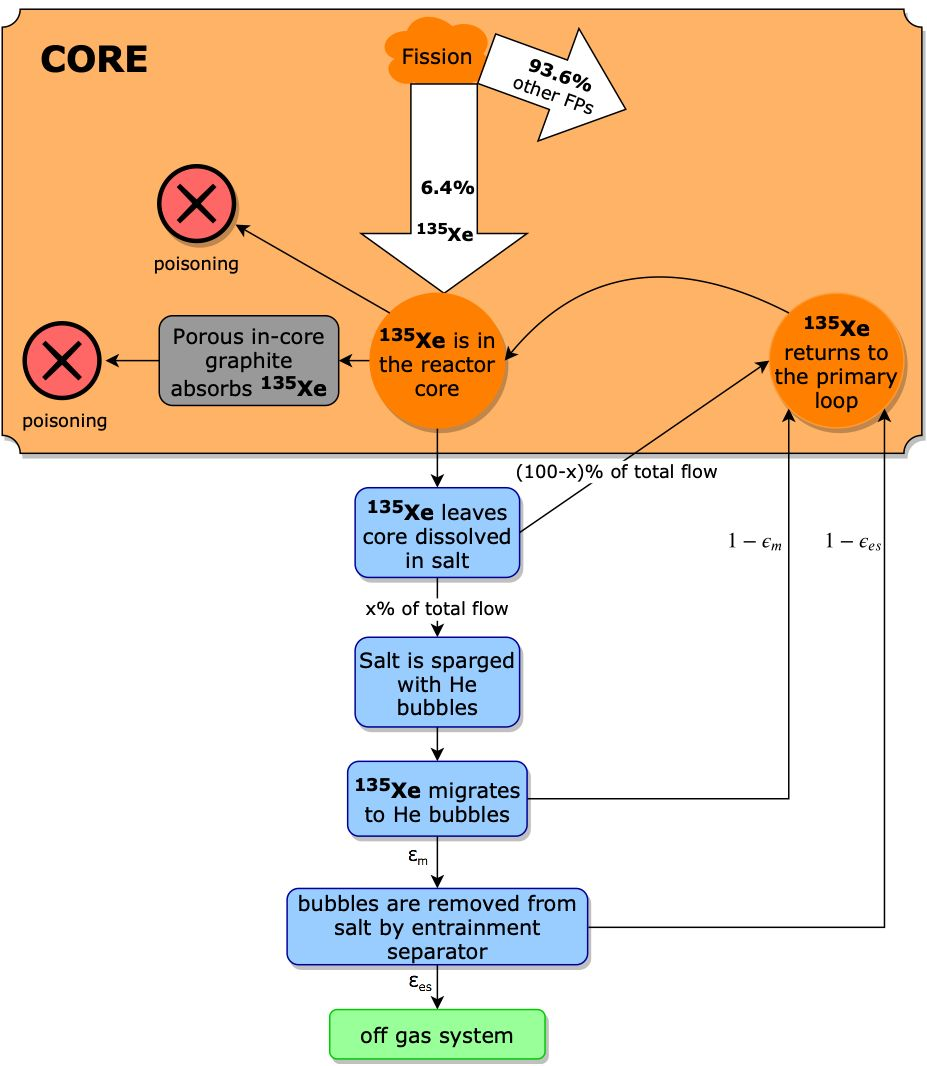
\includegraphics[width=0.6\textwidth]{principal_scheme.png}
        \end{center}
        \caption{Principal scheme of xenon removal from the salt.}
        \label{fig:scheme}
    \end{figure}

\subsubsection{Dakota}

    We used the Dakota code \cite{adams_dakota_2019} for sensitivity analysis to
    assess the reactor performance at different load-follow scenarios when the sparging system is enabled. The code provides optimization tools including senstivity analysis packages for miscellaneous design problems. With Dakota group's words:

    \begin{quote}
        "In addition to its state-of-the-art optimization methods, Dakota
        includes methods for global sensitivity and variance analysis, parameter
        estimation, uncertainty quantification, and verification, as well as
        meta-level strategies for surrogate-based optimization, hybrid
        optimization, and optimization under uncertainty."
    \end{quote}

    We performed multidimensional parameter study by computing response data sets for an n-dimensional hypergrid formed by sensitivity parameters. Each sensitivity parameter is partitioned into equally-spaced intervals between its upper and lower bounds. Each combination was then simulated by Saltproc software coupled with Serpent.

\subsubsection{Serpent}

    Serpent software \cite{Lep2014} was used for Monte-Carlo based neutron transport calculations. Serpent model with corresponding Serpent's parameters stand on MSBR design described in various reports prepared for ARPA-E MEITNER Program \cite{rykhlevskii_fuel_2019, rykhlevskii_modeling_2019, rykhlevskii_fuel_2020}.

\newpage
\FloatBarrier

\section{Sparging Design}

    A sparging system is composed of two separate components: Sparger (bubble generator) and Separator (bubble separator). A simple illustration of the system is given in Figure \ref{fig:sparging}.

    \begin{figure}[htbp!]
        \begin{center}
            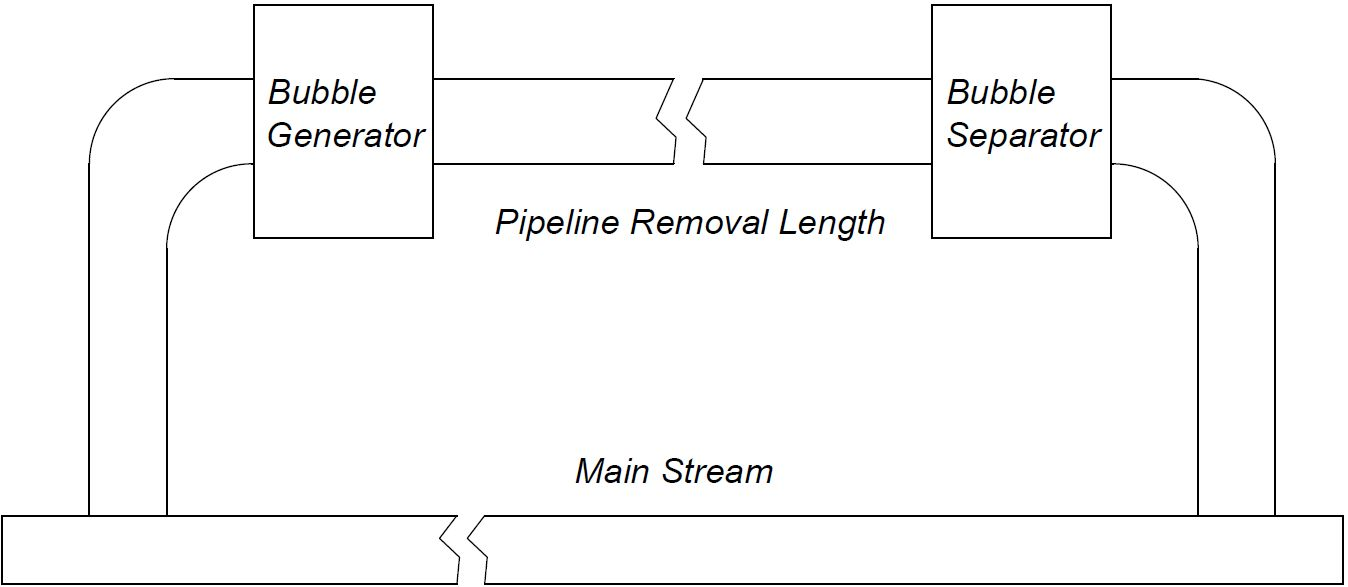
\includegraphics[width=0.8\textwidth]{bubble_separator_main.png}
        \end{center}
        \caption{Fission product removal system: Sparging}
        \label{fig:sparging}
    \end{figure}

\subsection{Sparger Design}

    The role of the sparger is to generate He bubbles which noble gases diffuse into. As illustrated in Figure \ref{fig:sparging}, sparger includes a contractor section and a long pipe with a contractor cross section of $A_c$ and length of $L$. Gas removal efficiency in bubble generator is defined by Eq. (2.1) based on \cite{peebles_removal_1968}.

    \begin{figure}[h!]
        \begin{center}
            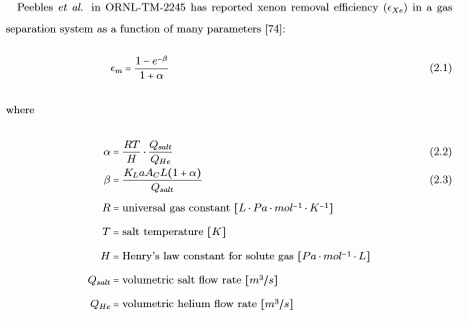
\includegraphics[width=1.0\textwidth]{eq2.1-part1.png}
            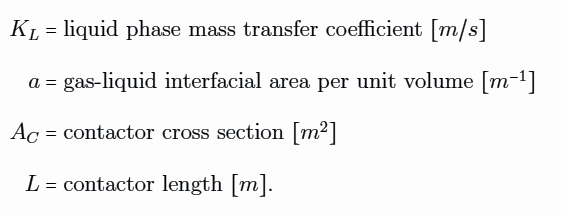
\includegraphics[width=0.6\textwidth]{eq2.1-part2.png}
        \end{center}
        \label{fig:eq2}
    \end{figure}

\newpage
\FloatBarrier

\subsection{Separator Design}

    A detailed design of the separator is given in Figure \ref{fig:bubble_sprt}. The role of the separator is to remove the bubbles from the fuel salt which carry volitale noble poisonous gases like Xe and Kr. Gas removal efficiency in bubble separator is defined by Eq. (6) reported by Gabbard report \cite{gabbard_development_1974}. In the equation, P is the pressure at the densitometer station, X is the gas injection rate, Qe is the liquid flow rate and Qg is the gas flow rate.

    \begin{figure}[htbp!]
        \begin{center}
            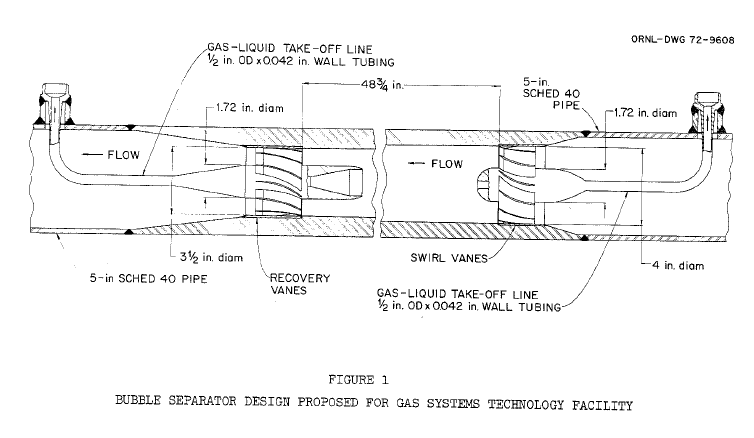
\includegraphics[width=\textwidth]{bubble_separator_detailed.png}
        \end{center}
        \caption{Entrainment Separator}
        \label{fig:bubble_sprt}
    \end{figure}

    \begin{figure}[htbp!]
        \begin{center}
            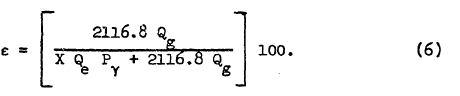
\includegraphics[width=0.7\textwidth]{eq6.png}
        \end{center}
        \label{fig:eq6}
    \end{figure}

\newpage
\FloatBarrier

\subsection{Integration to Saltproc}

    Sparging system was embedded to Saltproc by separately defining Sparger and Separator clasesses. \textit{read\_processes\_from\_input} function in \textit{app.py} script calls the classes to calculate removal efficiencies of target elements. More information about Saltproc functions and classes can be found in Milestone 2.1 report \cite{rykhlevskii_milestone_2019} and ARFC Github repo (https://github.com/arfc/saltproc). Sparger class uses Eq. 2.1 whereas Separator uses Eq. 6. In this way, besides existing flexibility, saltproc now enables Sparging system when "self" input key used in the json object file.

    Later, these equations will be modified by the experimental and simulation data to be supplied by the project research groups.

\newpage
\FloatBarrier

\section{Sensitivity Analysis}

    To design a feasible sparging system, we performed two separate sensitivity analyses:

    \begin{itemize}
        \item Reactor core behiour at different load-follow transient and decision to how much removal efficency is needed to maintain the critacilty in MSRE when the sparging system is enabled.
        \item Estimation of design boundaries and optimization of these design parameters.
    \end{itemize}

\subsection{Load-Follow}

    Figure \ref{fig:workflow} illustrates a simplified workflow of sensitivity analysis for reactor core behaviour. Results define $\varepsilon$$_{Xe}$
    requirements for prototype Xe sparger and entrainment separator system.

    \begin{figure}[htbp!]
        \begin{center}
            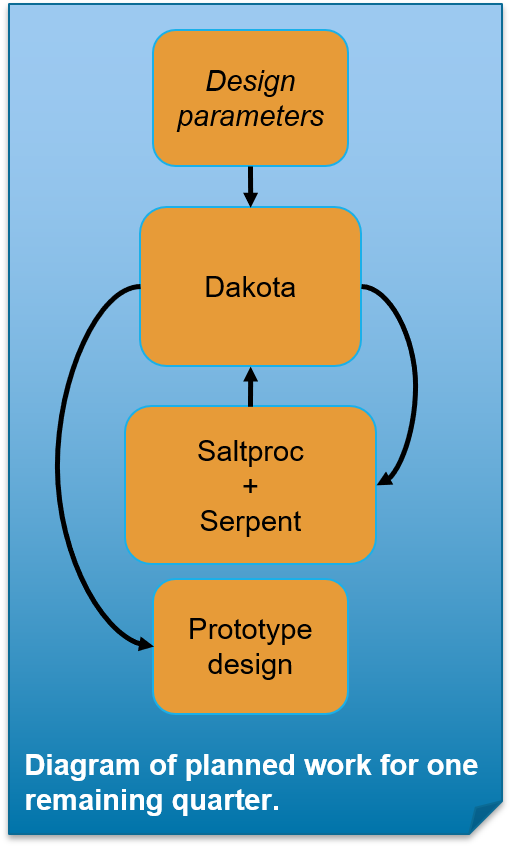
\includegraphics[width=0.35\textwidth]{workflow.png}
        \end{center}
        \caption{Sensitivity analysis workflow.}
        \label{fig:workflow}
    \end{figure}

\subsubsection{Scenarios}

    Two critical load following scenarios were investigated:
    \begin{itemize}
        \item The first worst case scenario simulates 8 hours at full power
        after an 8-hour shutdown, providing maximum Xe poisoning effect in the
        reactor.
        \item The second worst case scenario considers a short period load
        follow for maximum Xe accumulation over time. In this scenario,
        the reactor runs at full power for one hour after an hour of shutdown,
        and this repeats several times.
    \end{itemize}

\subsubsection{Sensitivity Parameters}

    Design parameters are selected as the total Xe removal efficiency
    ($\varepsilon$$_{Xe}$) by using Eq. 2.1 \cite{rykhlevskii_fuel_2020} in
    Figure \ref{fig:eq2}. $\varepsilon$$_{Xe}$ ranges from 0 to 100 \%.
    Performance metrics are considered to be k$_{eff}$, $\beta$$_{eff}$,
    breeding ($\gamma$) and reactivity feedbacks ($\alpha$).

    Other parameters defined by Eq 2.1 are as follow: length (L) = 11 m,
    diameter (d) = 0.4 m, volume (V) = 1.4 m$^{3}$, A$_c$ = 0.126 m$^{2}$, He
    bubble diameter, d$_b$ = 0.508 mm, salt volumetric flow rate (Q$_{salt}$) =
    2 m$^{3}$/s, sparging gas (helium) volumetric flow rate (Q$_{He}$) = 0.1
    m$^{3}$/s.

    Removal efficiency of any target isotopes in the separator is assumed 100 \%.

\subsection{Sparging System}

    As a final step of the sensitivity analysis for sparging system, we bounded
    sparging system design based on the load-following results.  For bubble
    generator and separator, we explored the effect of sensitivity (design)
    parameters on gas removal efficiencies of Xe, Kr and H target elements.

    To understand the interdependencies of design paramaters, we examined individual and binary effects of sparger design parameters on the Xe removal efficiency.

\subsubsection{Sensitivity Parameters}

    Design parameters for sparging system were considered as salt volumetric
    flow rate ($Q_{salt}$), helium volumetric flow rate ($Q_{He}$), bubble
    diameter ($d_b$), contractor pipe diameter ($d$), contractor pipe length
    ($L$), and salt temperature ($T_{salt}$). The metrics corresponding to the
    performance of the system are gas removal efficiencies ($\varepsilon$$_{X}$)
    of sparger and separator where $_{X}$ denotes Xe, Kr and H target elements.

    Base design parameters used in the sensitivity analysis for comparison are
    as follow: pipe length (L) = 10 m, pipe diameter ($d$) = 0.1 m, bubble
    diameter ($d_b$) = 1 mm, salt volumetric flow rate (Q$_{salt}$) = 0.1
    m$^{3}$/s, salt temperature ($T_{salt}$) = 900 K and helium volumetric flow
    rate (Q$_{He}$) = 5\% of the salt volumetric flow rate = 0.005 m$^{3}$/s.
    Accordingly, we changed these parameters between -50\% and +50\% (i.e.,
    $\pm$10\%, $\pm$25\% and $\pm$50\%).

\newpage
\FloatBarrier

\section{Results}

\subsection{Load-Follow}

    Initial results shown in Figure \ref{fig:loadfollow} and the results from
    previous work \cite{rykhlevskii_fuel_2020} point out that MSBR cannot do
    load-follow without gas removal at BOL (30 days), MOL (15 years) and EOL (30
    years) as the effective multiplication factor decreases with the start of
    shutdown. Although the online gas removal from the fuel salt even with moderate efficiency significantly reduces the xenon poisoning effect, very high removal efficiency seems unnecessary to negate the negative effect of xenon poisoning. Load-follow at EOL is the worst for k$_{eff}$ and consequently considered for sensitivity analysis.

    \begin{figure}[h]
        \begin{center}
            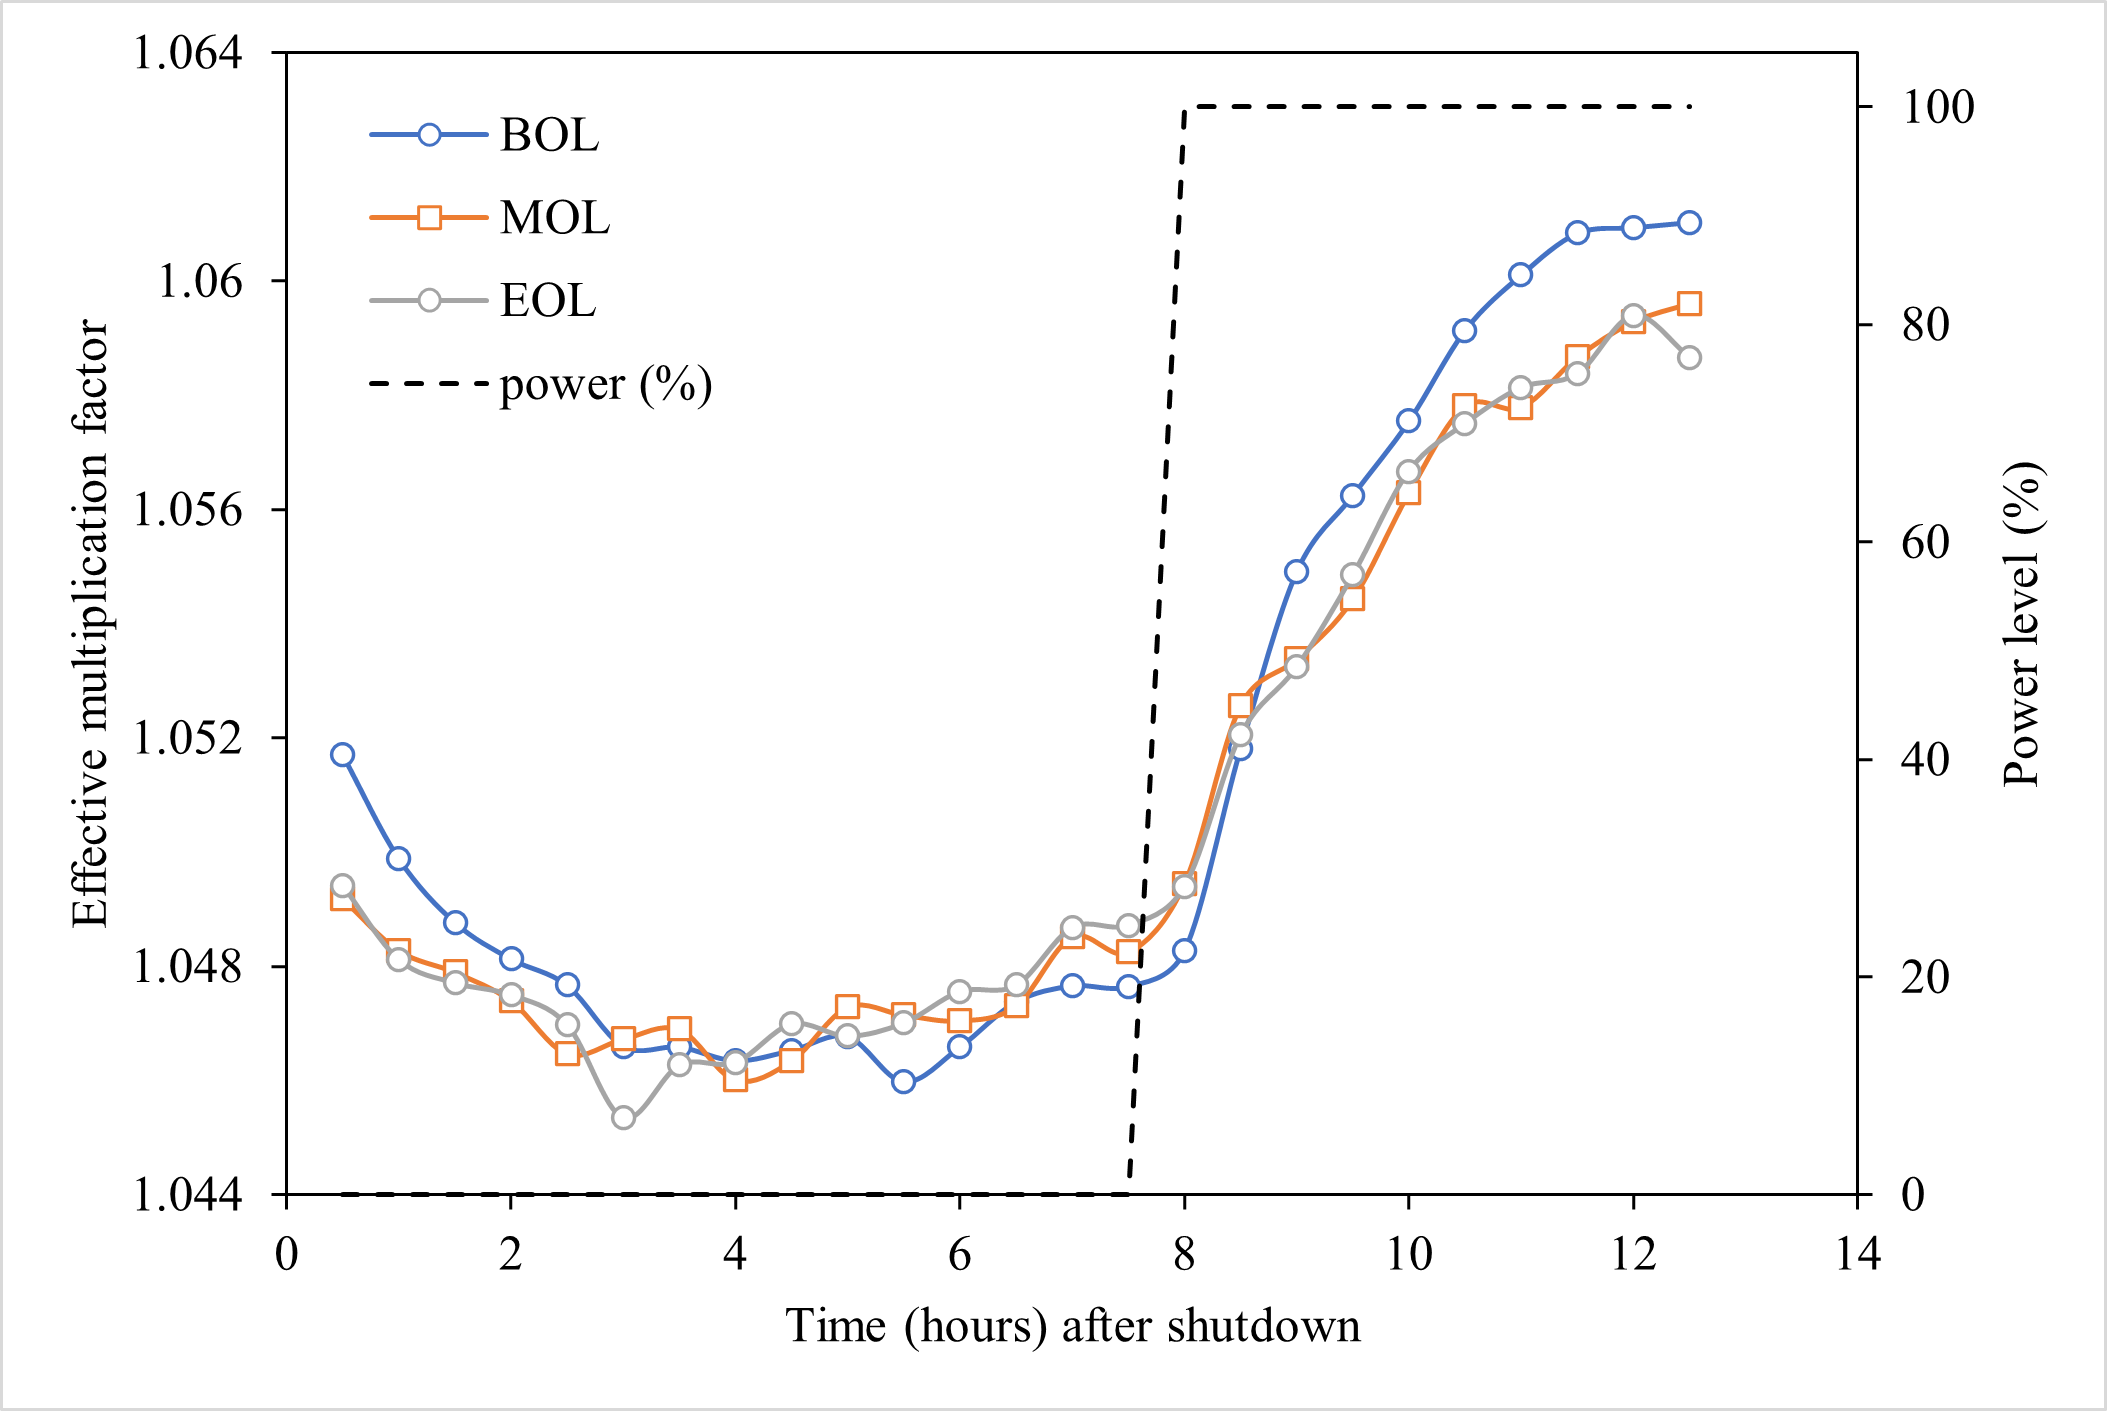
\includegraphics[width=1.0\textwidth]{msbr_loadfollow.png}
        \end{center}
        \caption{Load follow is attempted at BOL (30 days), MOL (15 years) and EOL (30 years) without gas removal system. Uncertainty in k$_{eff}$ is 25 pcm. 30 mins time resolution.}
        \label{fig:loadfollow}
    \end{figure}

\subsubsection{First Scenario}

    Figure \ref{fig:single_keff} shows the results of the first scenario for
    k$_{eff}$. After a lifetime of operation at $\varepsilon$$_{Xe}$ = 0.536,
    single load follow is attempted. In this transient, for the base case
    geometry, if $\varepsilon$$_{Xe}$ = 26.8\%, then the poisoning effect of Xe
    can be sufficiently negated. Generally, increasing gas removal efficiency
    increases excess reactivity. If higher efficiency is used, then the reactor
    can recover excess reactivity within a few hours for all
    $\varepsilon$$_{Xe}$ $>$ 26.8\% in base case geometry.

    As to breeding ratio depicted in Figure \ref{fig:single_breed}, single load
    following results in a gradual decrease. Increasing the gas removal
    efficiency slightly lowers the breeding ratio during load following.

    For the delayed neutron fraction ($\beta$$_{eff}$) given in Figure
    \ref{fig:single_delayed}, we observed no significant change. Instead,
    $\beta$$_{eff}$ fluctuates in a narrow range.

    We also explored multiple consecutive load follow transients to reveal the
    behavior of performance metrics under sharp changes in salt composition. As
    can be clearly seen in Figure \ref{fig:double_keff}, k$_{eff}$ begins
    fluctuating with Xe buildup and burndown period. We understand from the
    result that to keep the reactor stable, gas removal efficiency at least
    $\varepsilon$$_{Xe}$ = 53.6\% is required (corresponds in base case geometry
    to K$_{L}$ $>$ 25 ft/hr = 2.117 mm/s)

    When we add more transients with the same load follow period, we see from
    Figure \ref{fig:triple_keff} that a higher gas removal efficiency (at least
    $\varepsilon$$_{Xe}$ = 76.9\% or K$_{L}$ $>$ 50 ft/hr = 4.233 mm/s) is
    needed to keep the reactor stable. Therefore, these results imply that as
    the number of power ramps increases, a higher gas removal efficiency is
    required for stable behavior.

    \begin{figure}[htbp!]
        \begin{center}
            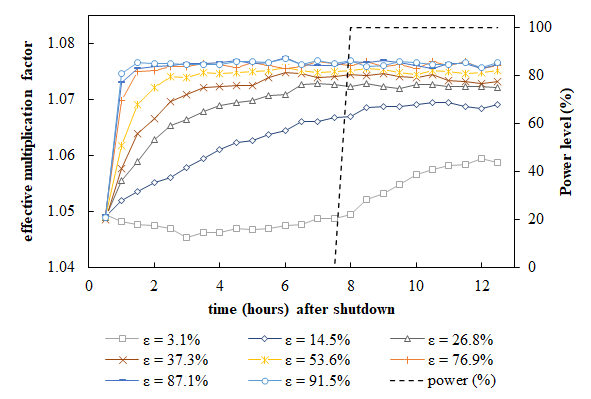
\includegraphics[width=0.8\textwidth]{single_ramp_keff.png}
        \end{center}
        \caption{After a lifetime of operation at $\varepsilon$$_{Xe}$= 0.536, load follow is attempted at EOL. Above shows k$_{eff}$ during load follow transient for various total Xe removal efficiencies
        ($\varepsilon$$_{Xe}$) over time after shutdown.}
        \label{fig:single_keff}
    \end{figure}

    \begin{figure}[htbp!]
        \begin{center}
            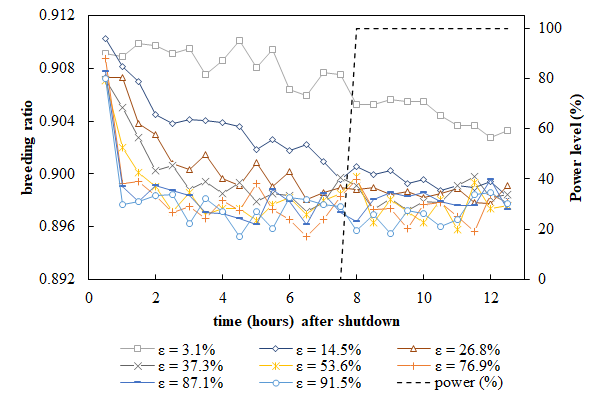
\includegraphics[width=0.8\textwidth]{single_ramp_breeding.png}
        \end{center}
        \caption{After a lifetime of operation at $\varepsilon$$_{Xe}$= 0.536, load follow is attempted at EOL. Above shows breeding ratio during load
        follow transient for various total Xe removal efficiencies
        ($\varepsilon$$_{Xe}$) over time after shutdown.}
        \label{fig:single_breed}
    \end{figure}

    \begin{figure}[htbp!]
        \begin{center}
            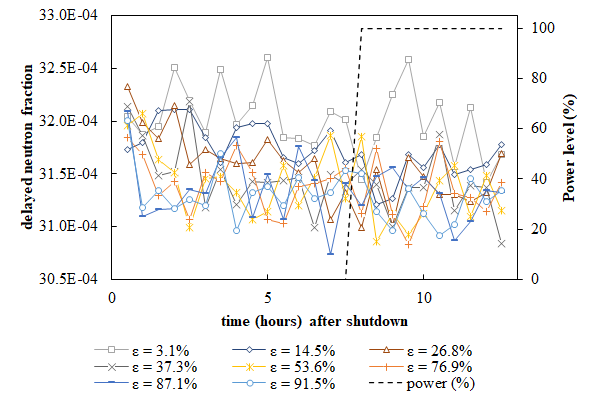
\includegraphics[width=0.8\textwidth]{single_ramp_delayed.png}
        \end{center}
        \caption{After a lifetime of operation at $\varepsilon$$_{Xe}$= 0.536, load follow is attempted at EOL. Above shows $\beta$$_{eff}$ during load
        follow transient for various total Xe removal efficiencies
        ($\varepsilon$$_{Xe}$) over time after shutdown.}
        \label{fig:single_delayed}
    \end{figure}

    \begin{figure}[htbp!]
        \begin{center}
            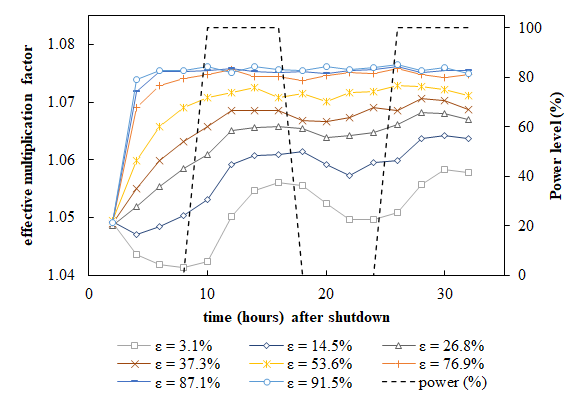
\includegraphics[width=0.8\textwidth]{double_ramp_keff.png}
        \end{center}
        \caption{After a lifetime of operation at $\varepsilon$$_{Xe}$= 0.536, load follow is attempted at EOL. Above shows k$_{eff}$ during multiple load follow transient for various total Xe removal efficiencies
        ($\varepsilon$$_{Xe}$) over time after shutdown.}
        \label{fig:double_keff}
    \end{figure}

    \begin{figure}[htbp!]
        \begin{center}
            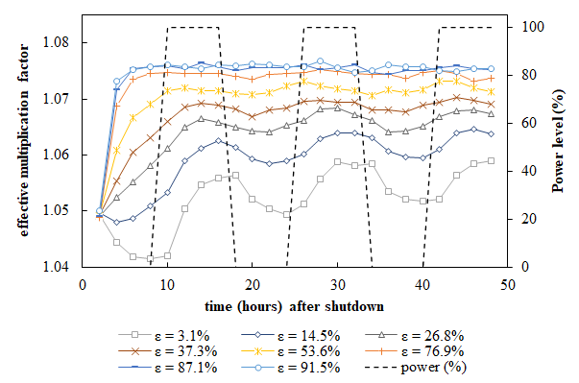
\includegraphics[width=0.8\textwidth]{triple_ramp_keff.png}
        \end{center}
        \caption{After a lifetime of operation at $\varepsilon$$_{Xe}$= 0.536, load follow is attempted at EOL. Above shows  k$_{eff}$ during multiple load follow transient for various total Xe removal efficiencies
        ($\varepsilon$$_{Xe}$) over time after shutdown.}
        \label{fig:triple_keff}
    \end{figure}

\newpage
\FloatBarrier

\subsubsection{Second Scenario}

    In the case of short period load following (second scenario), we implemented
    four consecutive power ramp. In this case, as can be seen in Figure
    \ref{fig:quadro_keff}, we see a quick recovery from shutdown even with low
    gas removal efficiency.

    \begin{figure}[htbp!]
        \begin{center}
            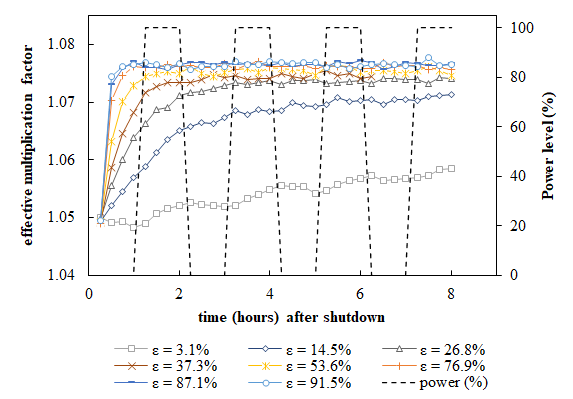
\includegraphics[width=0.9\textwidth]{quadro_ramp_keff.png}
        \end{center}
        \caption{After a lifetime of operation at $\varepsilon$$_{Xe}$= 0.536, load follow is attempted at EOL. Above shows  k$_{eff}$ during multiple load follow transient for various total Xe removal efficiencies
        ($\varepsilon$$_{Xe}$) over time after shutdown.}
        \label{fig:quadro_keff}
    \end{figure}

\newpage
\FloatBarrier

\subsection{Sparging System}

\subsubsection{Sparger Design}

    Figure \ref{fig:individual_eff_sparger} and \ref{fig:binary_eff_sparger}
    show change in Xe removal efficiency for sparger. When we look at the individual effects on sparger design, gas removal efficiencies decrease with increasing bubble diameter and salt flow rate whereas gas removal efficiencies increase with increasing pipe diameter, pipe length, helium flow rate and salt temperature. In addition, change of tritium removal efficiency somewhat different from that of Xe and Kr removal efficiency, being affected significantly by salt temperature change.

    Furthermore, salt temperature and sparger pipe diameter look like not
    effective players in the adjustment of the gas removal efficiency as the
    10\% increase in temperature only results in about 3\% increase in
    efficiency. Even with 50\% change, there is only 10\% gain in efficiency, by
    increasing from 40\% to about 45\%. In addition, we will need an additional
    heater before sparger to elevate the salt temperature as the salt
    temperature is determined by the reactor design itself.

    \begin{figure}[htbp!]
        \begin{center}
            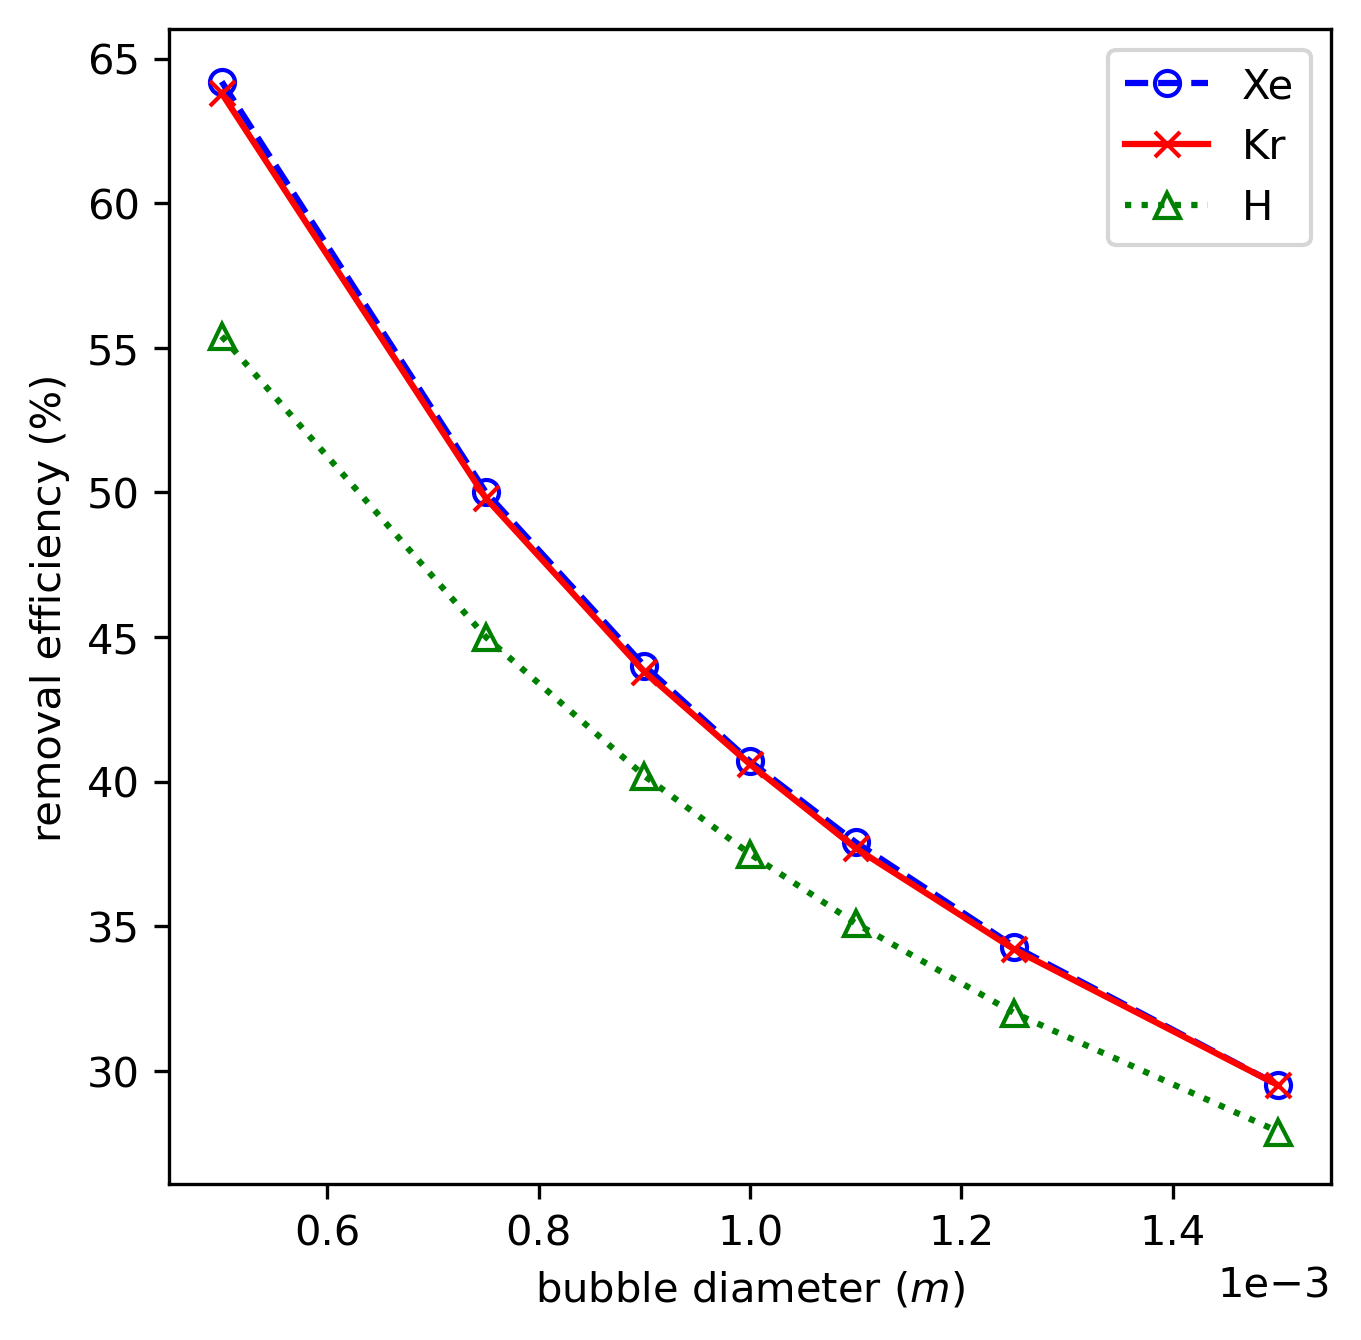
\includegraphics[width=0.45\textwidth]{Xe_eff_vs_db.png}
            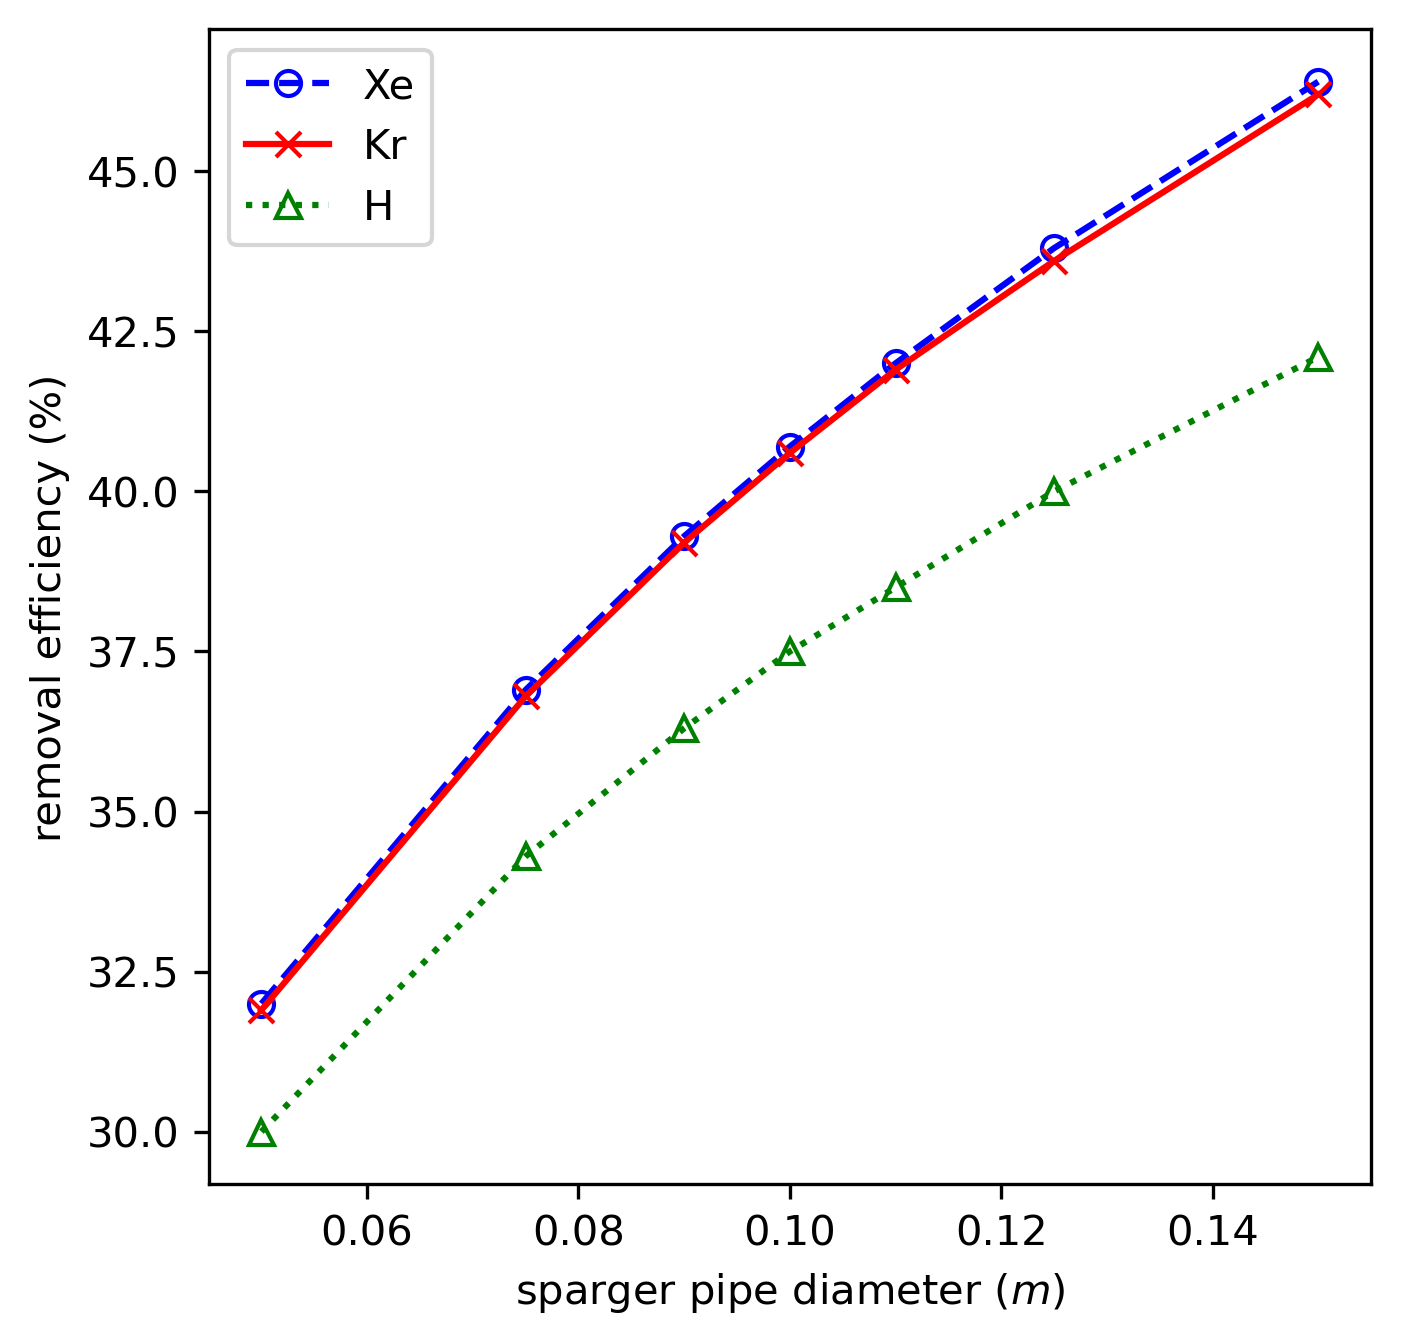
\includegraphics[width=0.45\textwidth]{Xe_eff_vs_ds.png}
            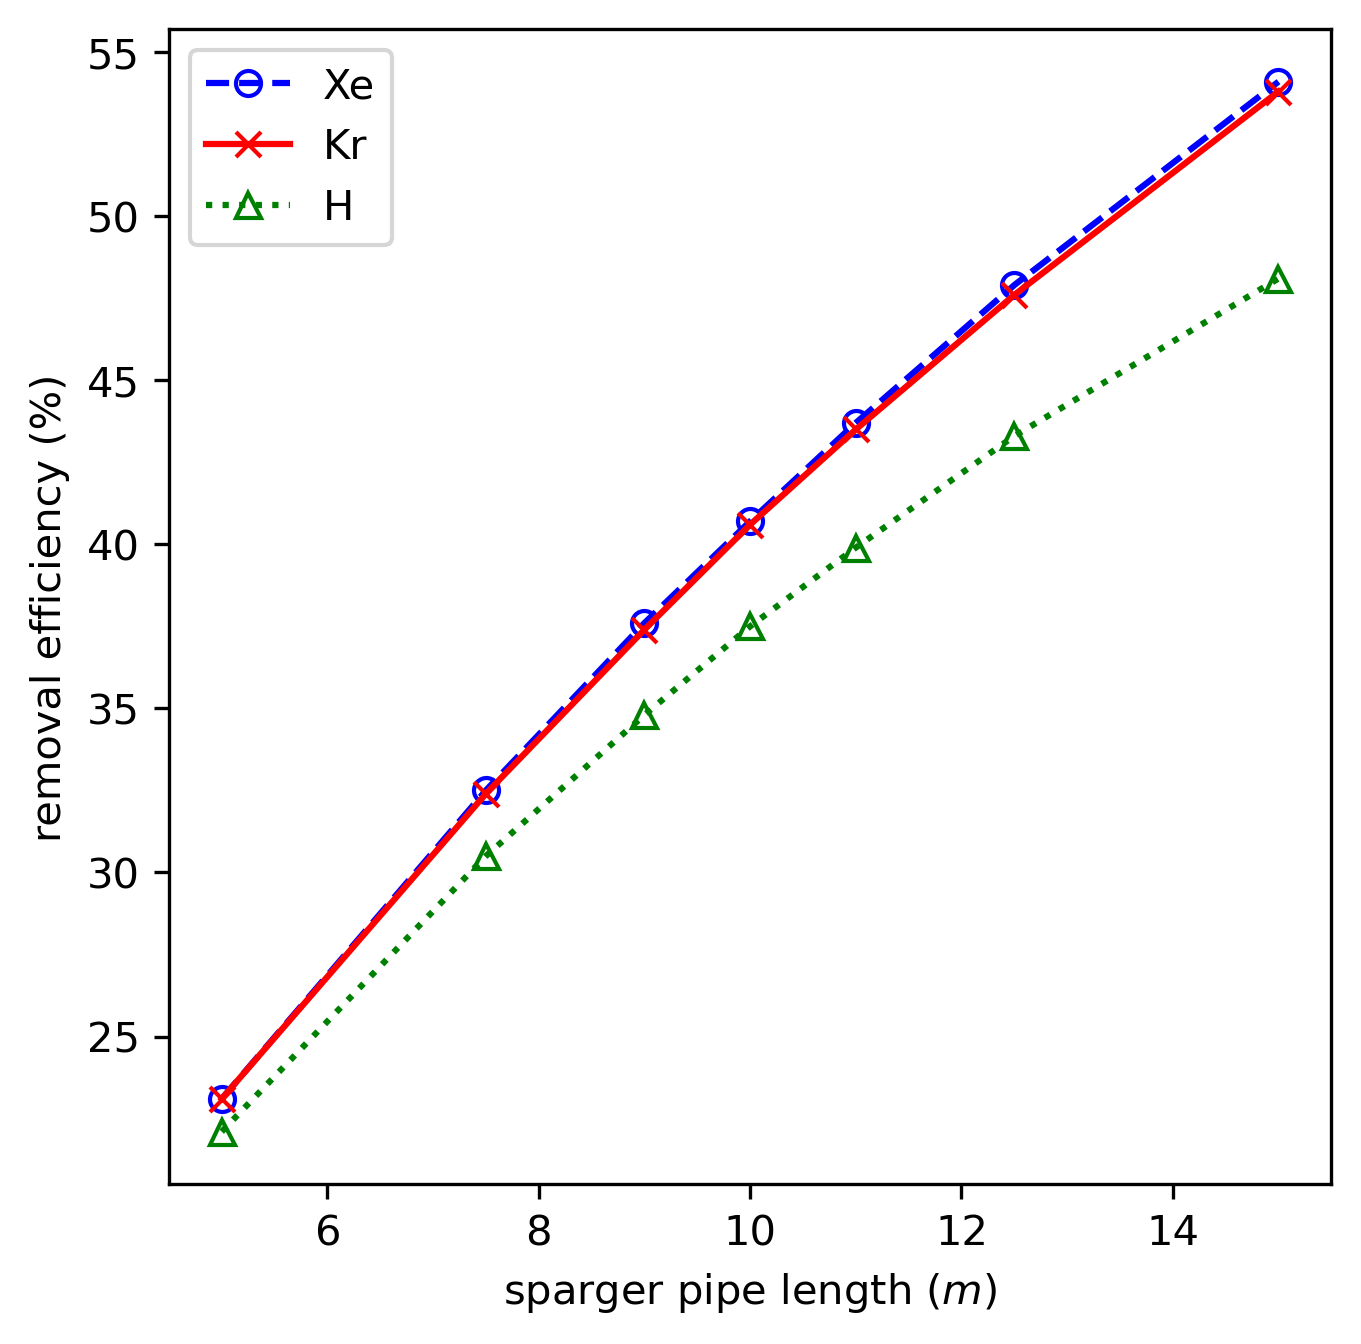
\includegraphics[width=0.45\textwidth]{Xe_eff_vs_L.png}
            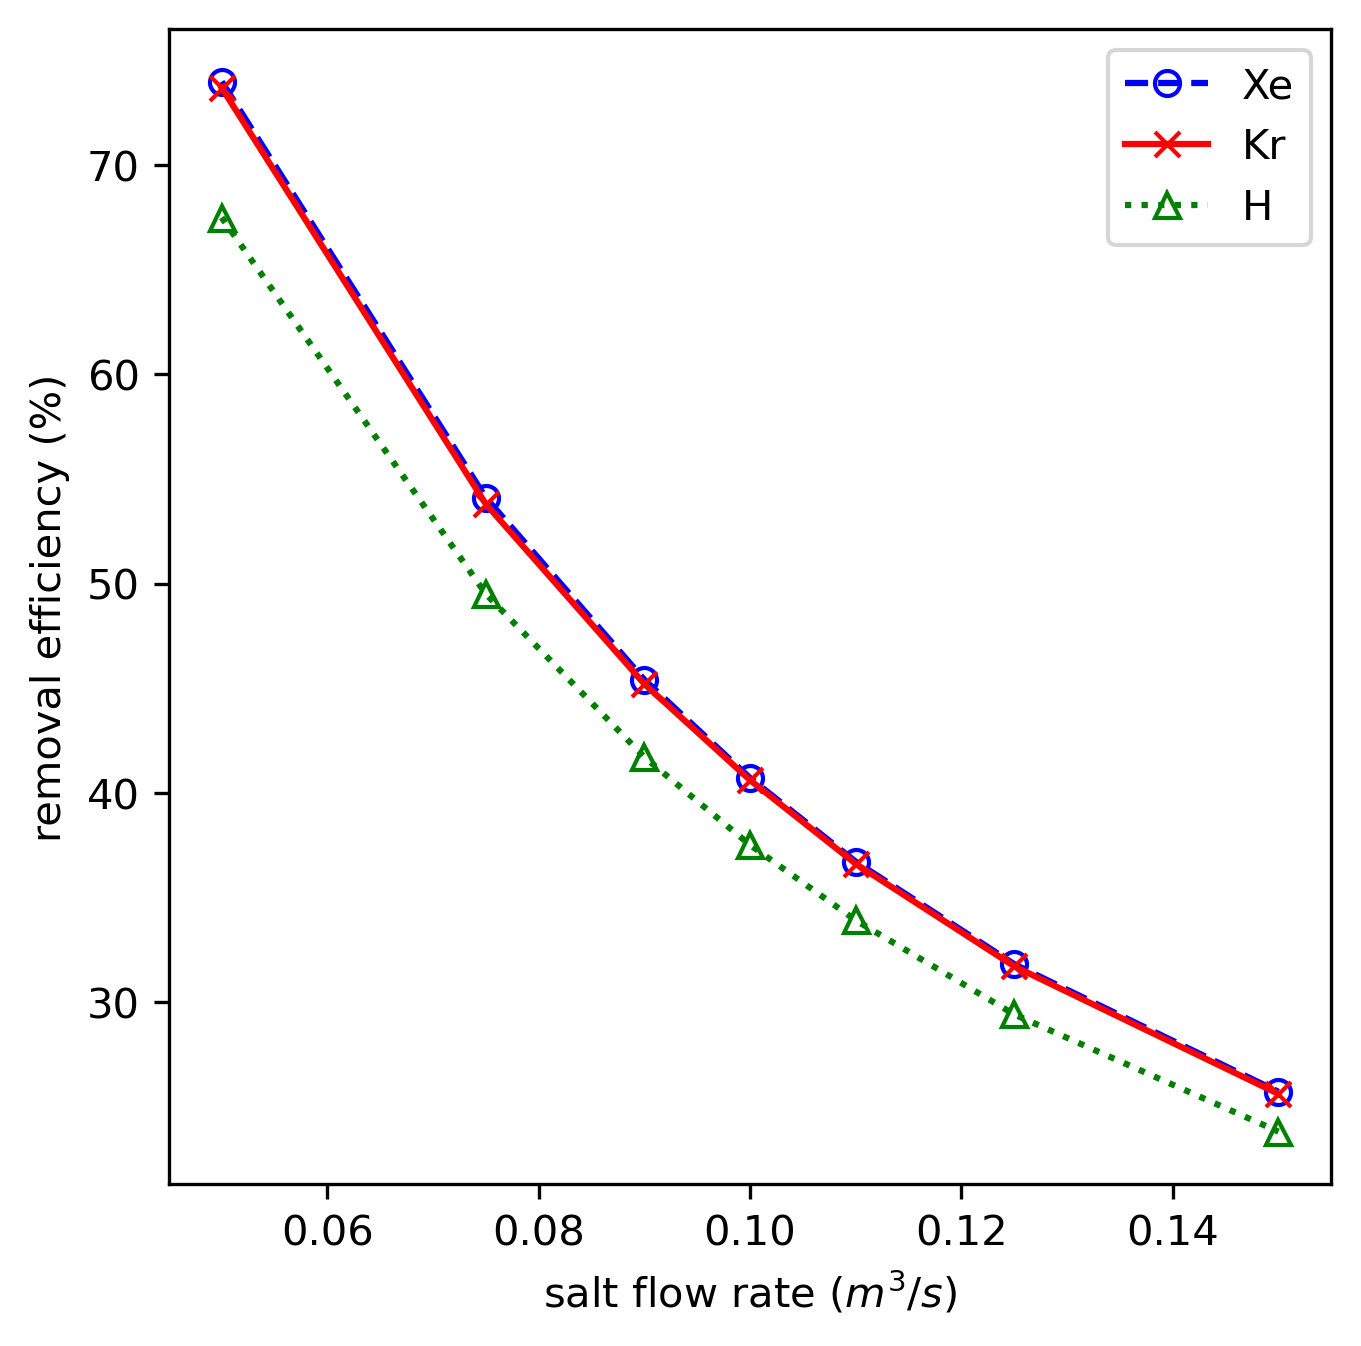
\includegraphics[width=0.45\textwidth]{Xe_eff_vs_Q_salt.png}
            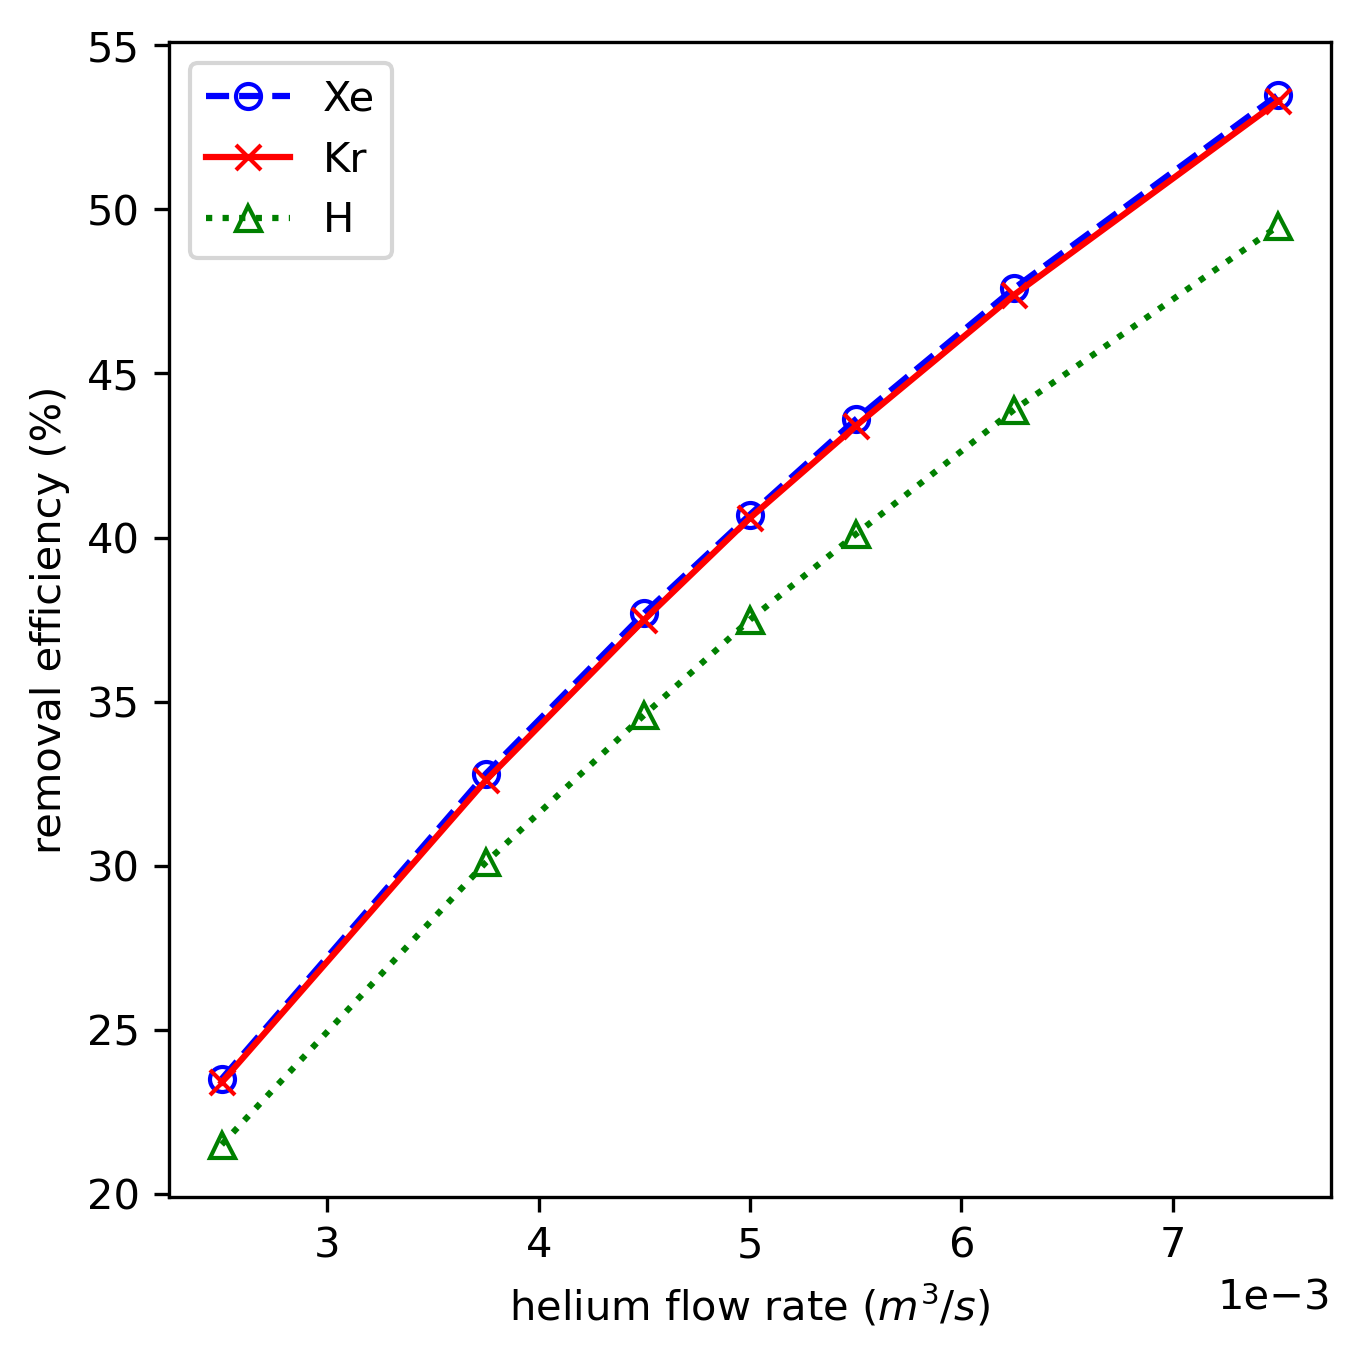
\includegraphics[width=0.45\textwidth]{Xe_eff_vs_Q_He.png}
            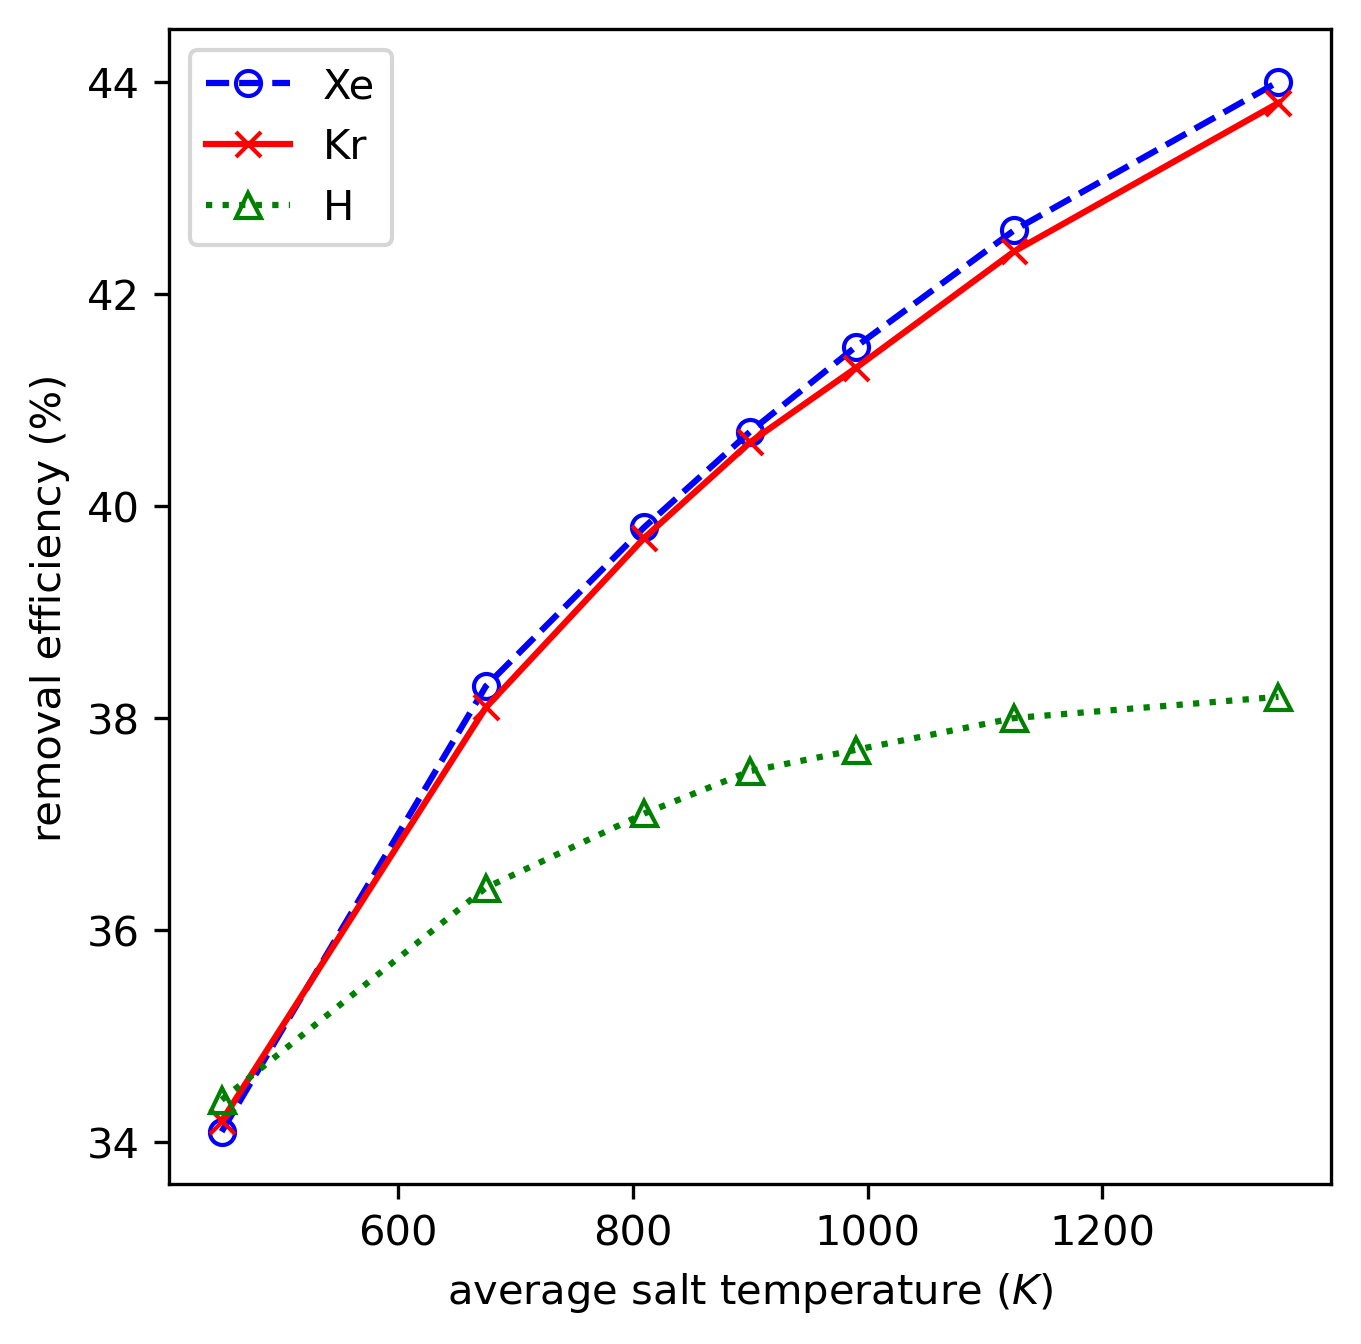
\includegraphics[width=0.45\textwidth]{Xe_eff_vs_Tsalt.png}
        \end{center}
        \caption{Individual effect of design parameters on Xe removal
            efficiency
            ($\varepsilon$$_{Xe}$) in sparger.}
        \label{fig:individual_eff_sparger}
    \end{figure}

    \begin{figure}[htbp!]
        \begin{center}
            \includegraphics[width=0.7\textwidth]{binary_eff_sparger.png}
        \end{center}
        \caption{Binary effect of design parameters on Xe removal
            efficiency
            ($\varepsilon$$_{Xe}$) in sparger.}
        \label{fig:binary_eff_sparger}
    \end{figure}

\newpage
\FloatBarrier

\subsubsection{Separator Design}

    Figure \ref{fig:individual_eff_separator} and \ref{fig:binary_eff_separator}
    show change in Xe removal efficiency for separator. According to the
    results, gas removal efficiency increases with increasing gas flow rate
    whereas it decreases with increasing other parameters.

    As discussed in Milestone 1.2 for the effect of bubble diameter on separator, bubble diameter has to be aroud 1 mm because both sparger and separator are influenced by it. The smaller bubble diameter the sparger has, the higher gas removal efficency the sparger provides. Oppositely, the smaller bubble diameter the separator has, the lower gas removal efficency the separator provides.

\begin{figure}[htbp!]
    \begin{center}
        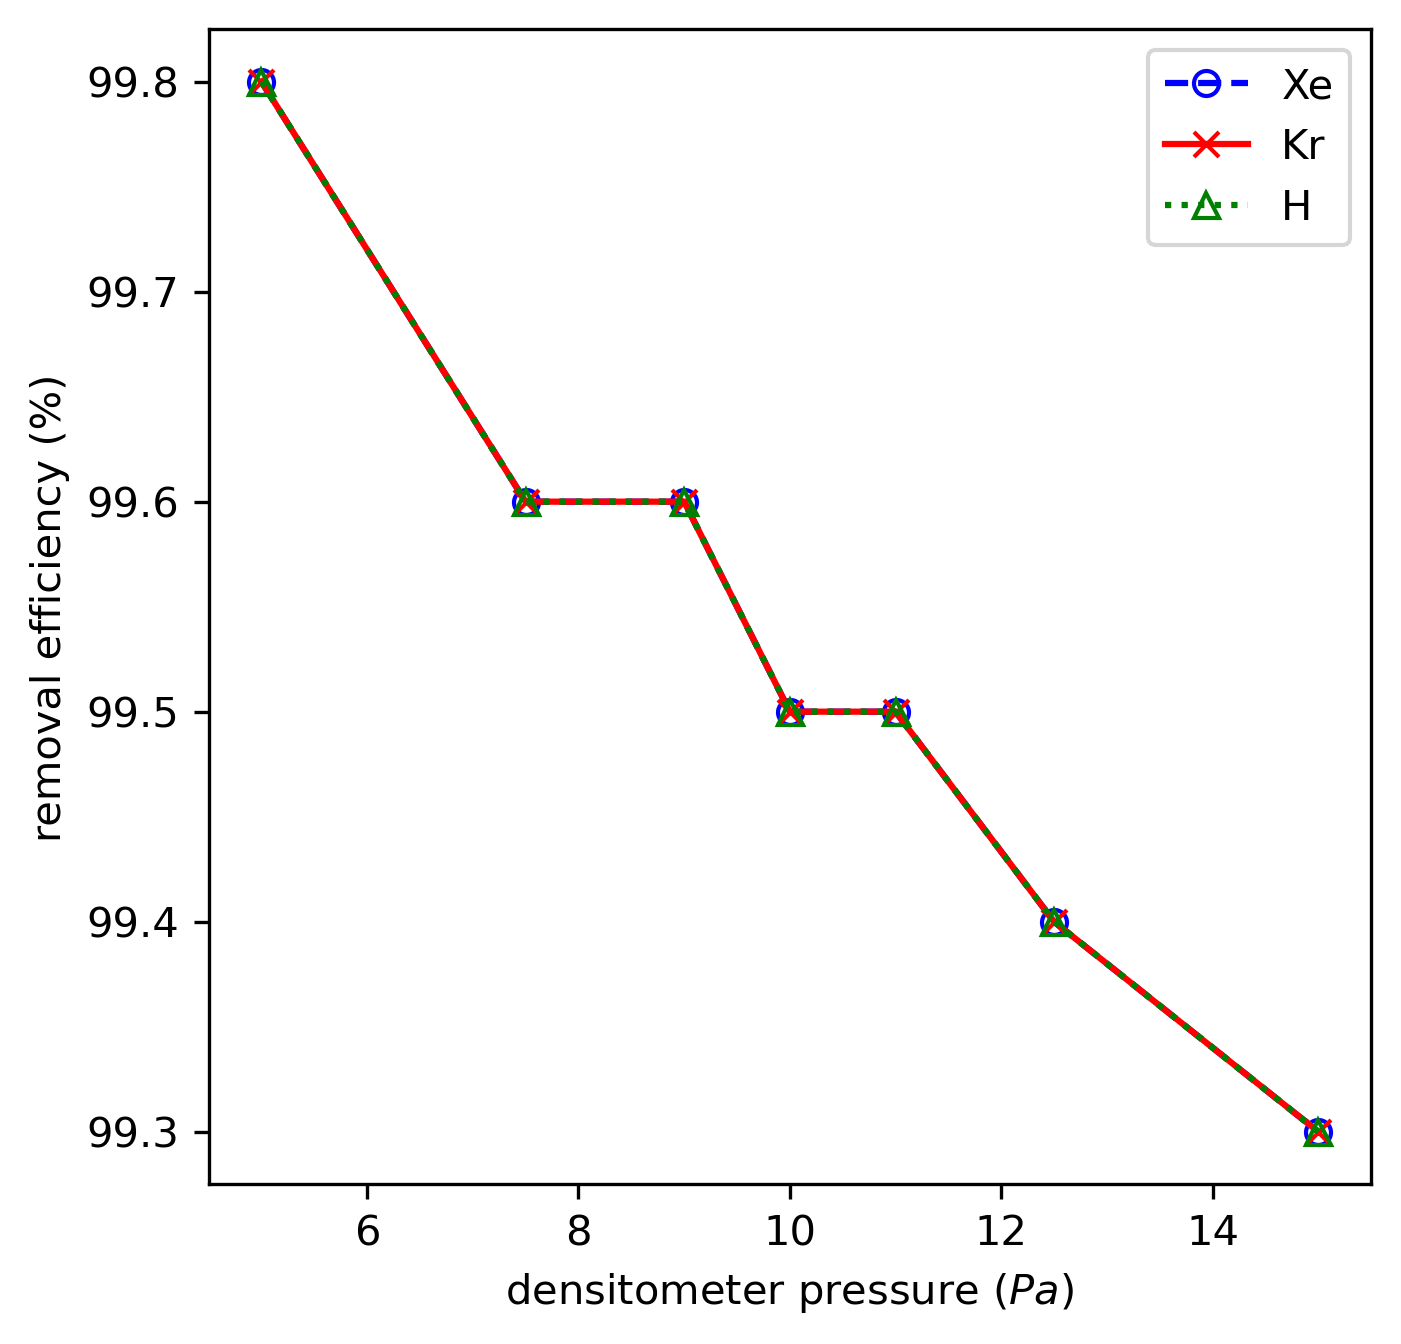
\includegraphics[width=0.45\textwidth]{Xe_eff_vs_Pgamma.png}
        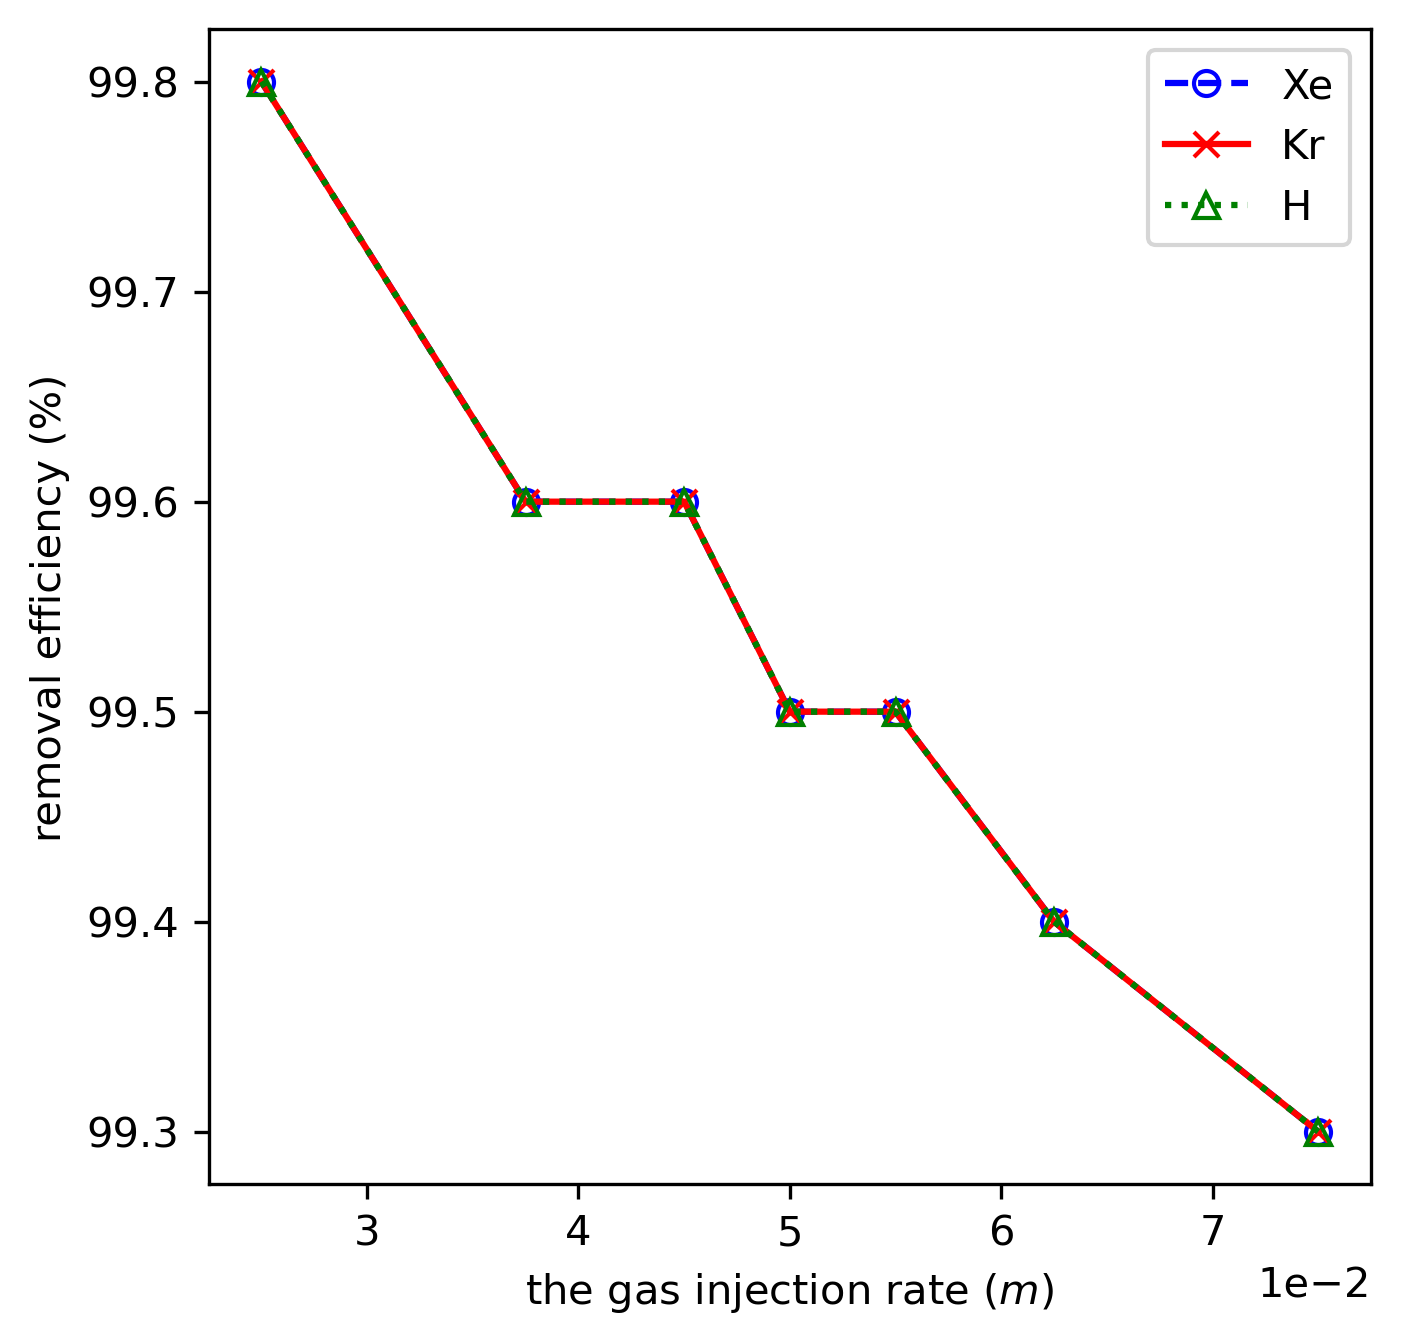
\includegraphics[width=0.45\textwidth]{Xe_eff_vs_X.png}
        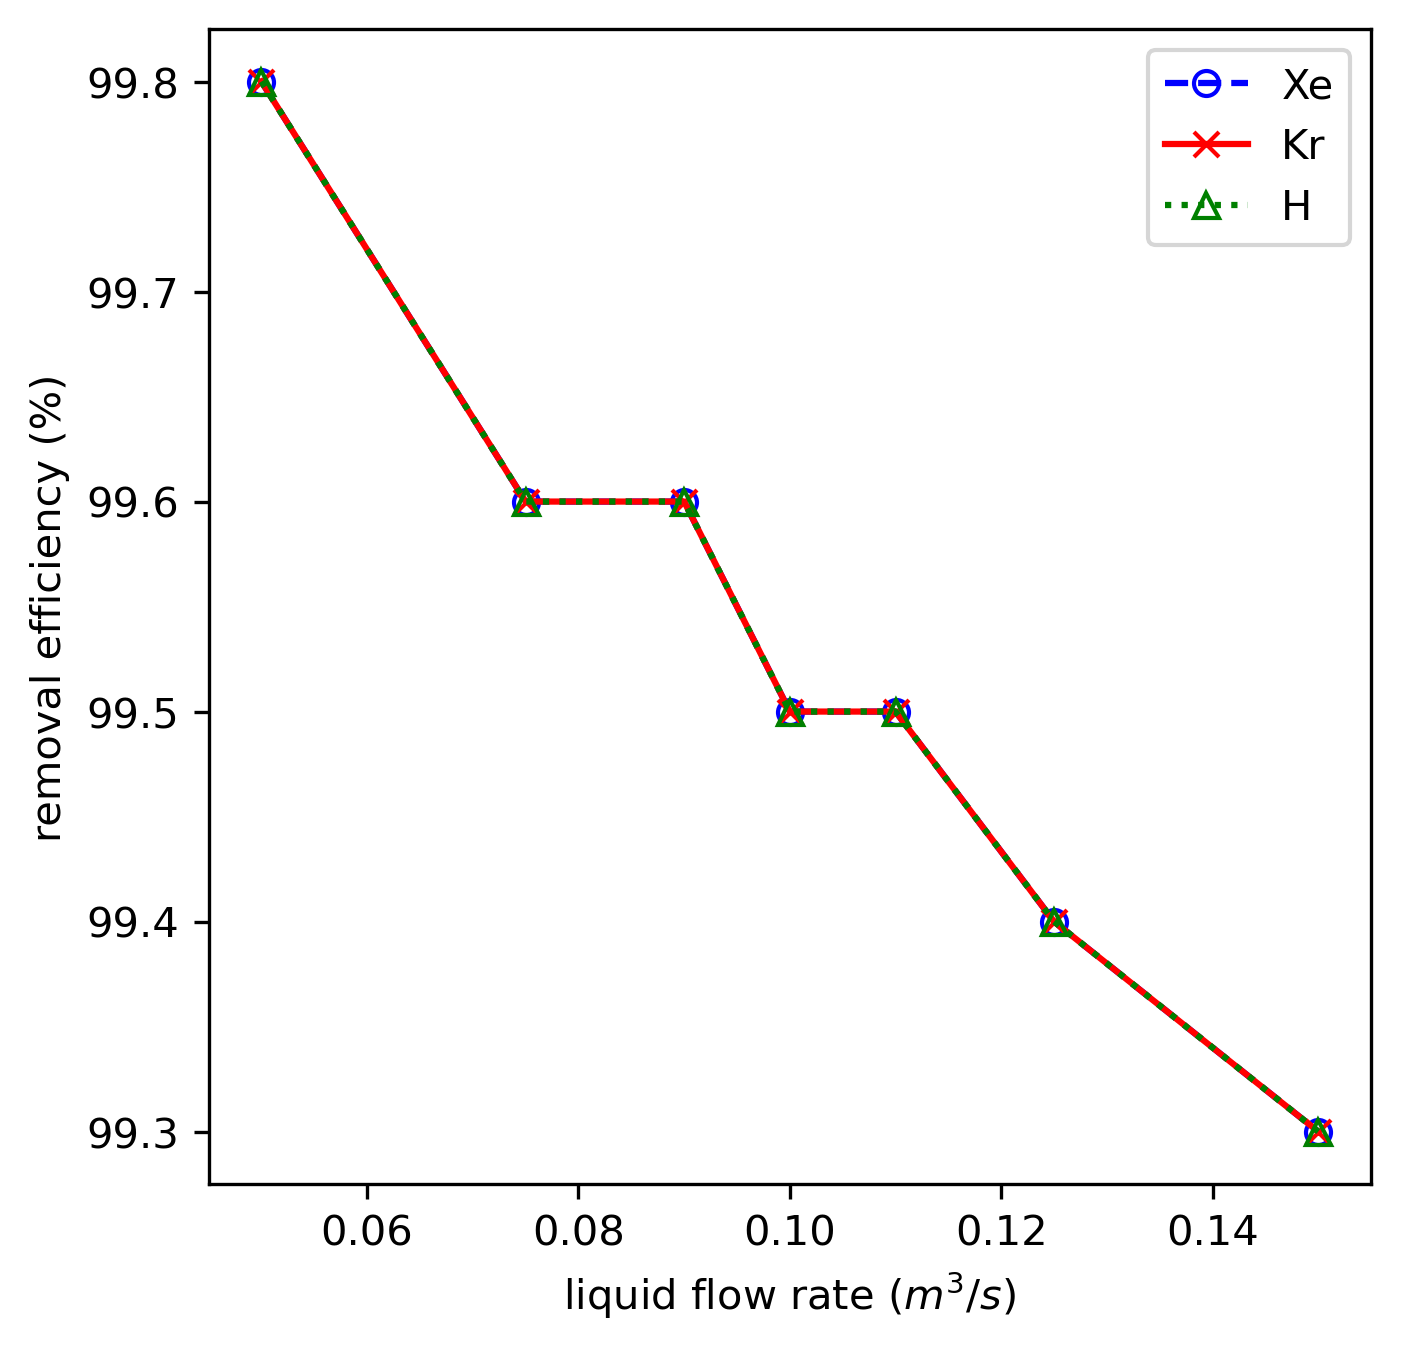
\includegraphics[width=0.45\textwidth]{Xe_eff_vs_Qe.png}
        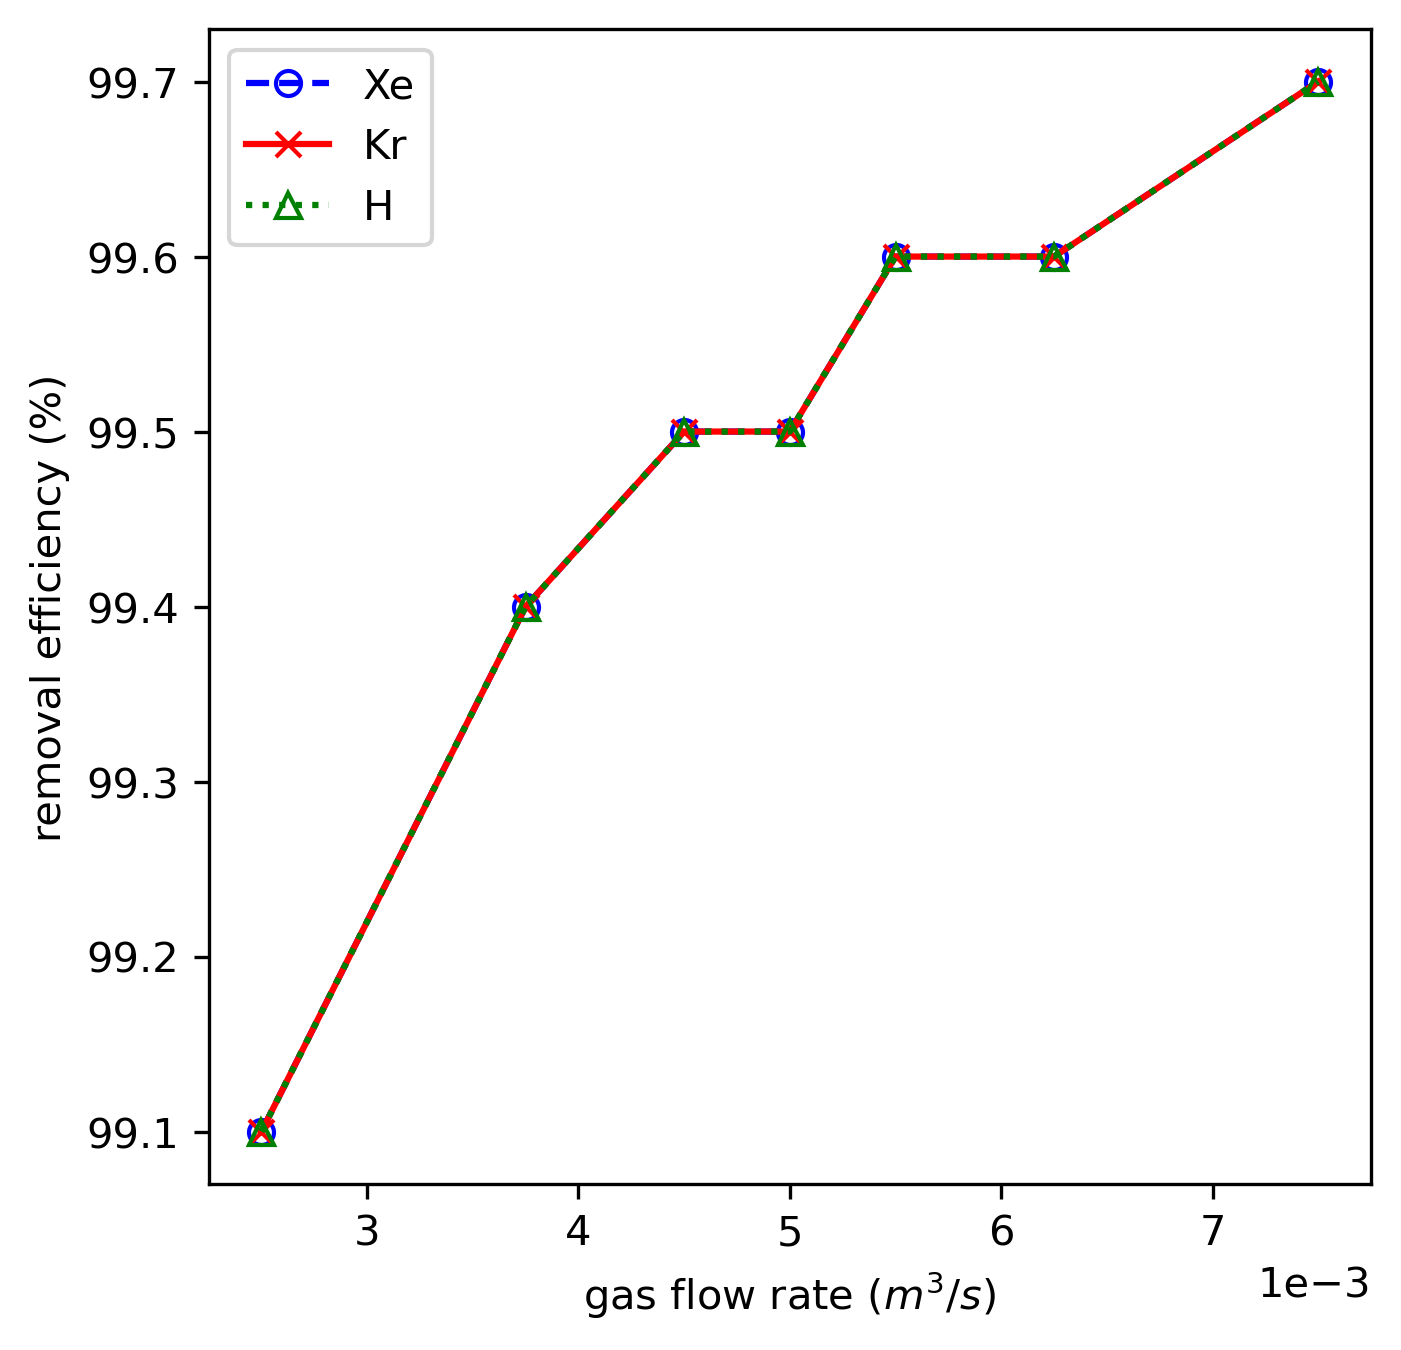
\includegraphics[width=0.45\textwidth]{Xe_eff_vs_Qg.png}
    \end{center}
    \caption{Individual effect of design parameters on Xe removal
    efficiency
        ($\varepsilon$$_{Xe}$) in separator.}
    \label{fig:individual_eff_separator}
\end{figure}

\begin{figure}[htbp!]
    \begin{center}
        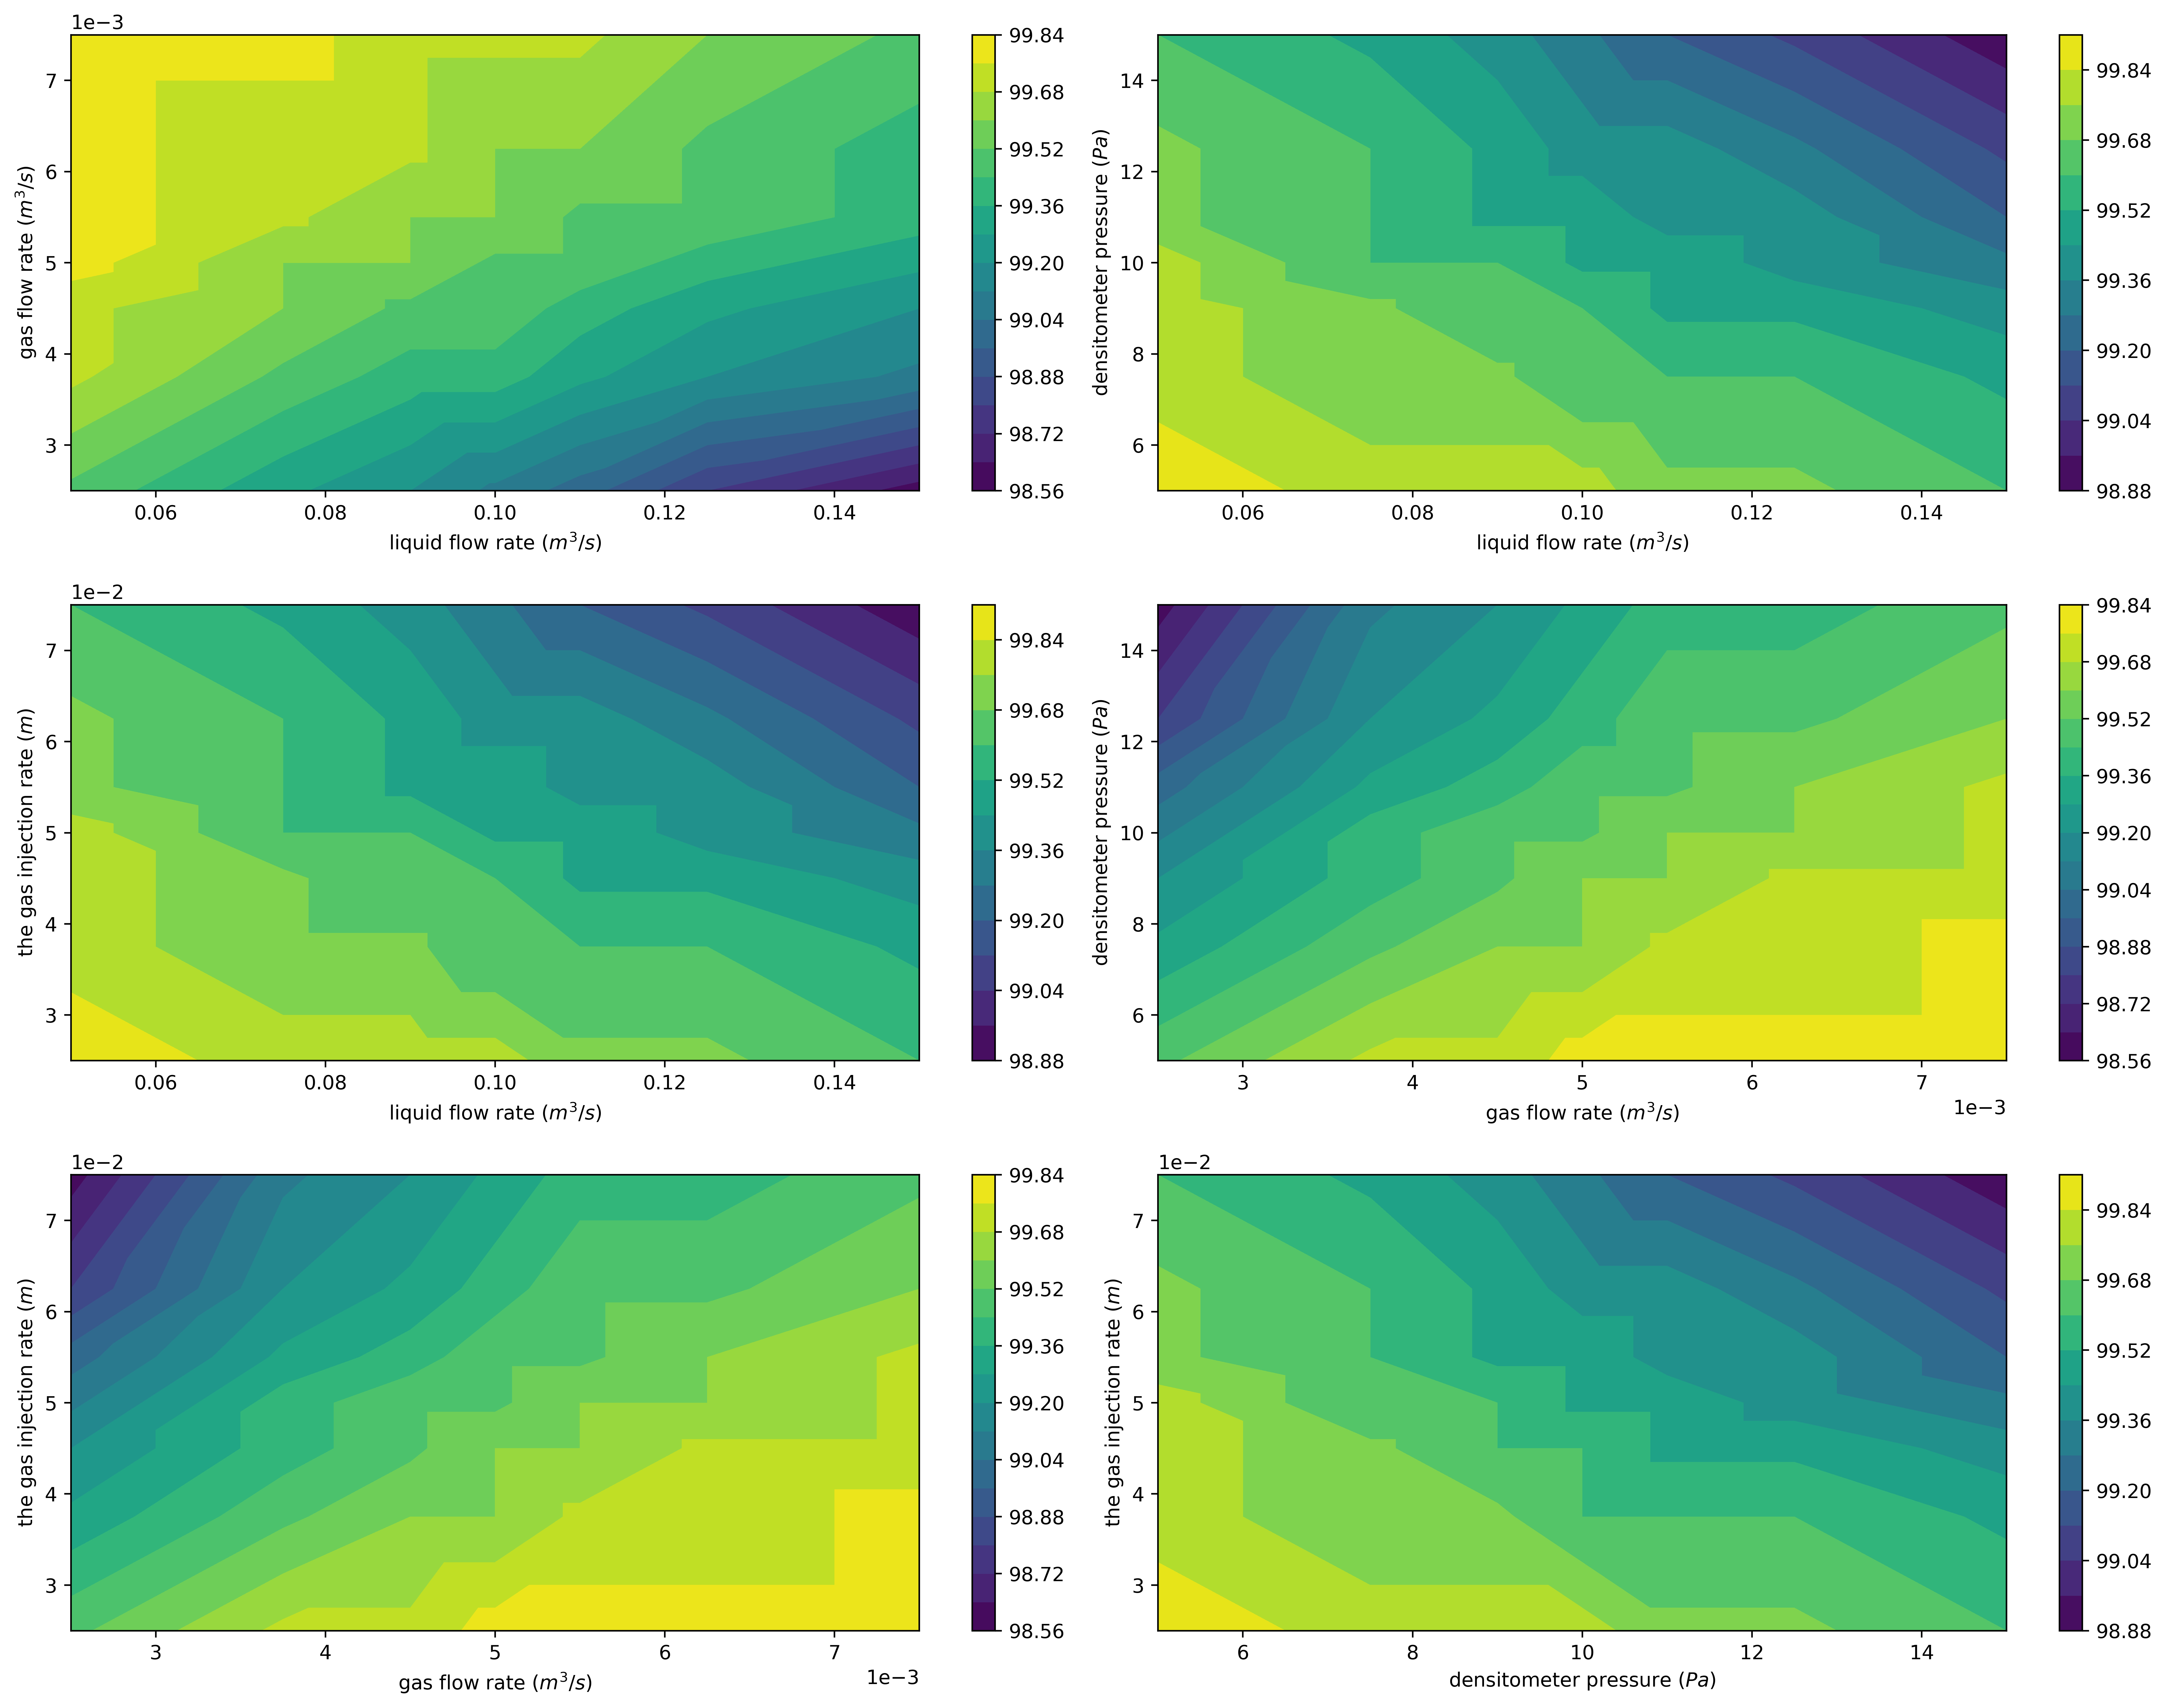
\includegraphics[width=1.0\textwidth]{binary_eff_separator.png}
    \end{center}
    \caption{Binary effect of design parameters on Xe removal
    efficiency
        ($\varepsilon$$_{Xe}$) in separator.}
    \label{fig:binary_eff_separator}
\end{figure}

\newpage
\FloatBarrier

\section{Conclusion}

    In short, MSBR can, without difficulty, operate under load follow transient
    with low gas removal efficiency, unless the shutdown period is too long,
    typically greater than 4 hours. Recovery time depends directly on gas
    removal efficiency and load-follow period.

    From the binary effects of the design parameters of sparger and separator, each design parameter has no relation with other parameters, acting like free variable and affecting the removal efficiency independently.

    Even if we change the separator design parameters by half, change in gas
    removal efficiency seems remaining limited, always higher than 99\%.
    Therefore, these results indicate that main diffficulty in desining sparging
    system comes from nothing but the sparger component. It has to be designed
    according to the removal efficiency imposed by the reactor core. Note that one of the important design parameters which is affecting both sparger and
    separator is bubble diameter as pointed out in Milestone 1.2.

    The base design which provides an $\varepsilon$$_{Xe}$ of about
    40\% may be a good starting point in designing sparging system. This design
    seems sufficient in particular for the reactor cores which needs less than
    40\% gas removal efficiency to compensate the reactivity loss due to Xe
    poisining. On the other hand, it is clear that we need a more adaptable
    sparger design for prompt response to a need for a higher gas removal
    efficiency like $\varepsilon$$_{Xe}$ = 0.769 as indicated in Figure
    \ref{fig:triple_keff}.

     It is appear from the results that the best option is to regulate the gas
    flow rate and/or salt flow rate during operation, or much better is to
    balance the ratio of gas flow rate to salt flow rate, which is delimited by
    thermal-hydralic effects as no higher than 5\%. Another good option is to
    make the sparger pipe length longer as efficiency reacts equally to change
    in length, like 10\% for 10\%. It also has no effect on separator.

    To reach at the goal of $\varepsilon$$_{Xe}$ = 53.6 implied by Figure
    \ref{fig:double_keff} for the double load follow transient, it would be
    sufficient to increase only sparger pipe length and diameter by 30\% in the
    base design, without touching the gas and salt flow rates. That is, the
    sparger design should have a pipe length (L) = 13 m, pipe diameter ($d$) =
    0.13 m, bubble diameter ($d_b$) = 1 mm, salt volumetric flow rate
    (Q$_{salt}$) = 0.1 m$^{3}$/s, salt temperature ($T_{salt}$) = 900 K and
    helium volumetric flow rate (Q$_{He}$) = 0.005 m$^{3}$/s.

    In the case of reaching at the goal of $\varepsilon$$_{Xe}$ = 76.9\% implied
    by Figure \ref{fig:triple_keff} for the triple load follow transient, it
    would not be as easy as to go the goal of $\varepsilon$$_{Xe}$ = 53.6\%.
    This is because there is no way to go to 76.9\% even if we increase the
    sparger pipe length and diameter by 50\%. Therefore we need additional
    parameters to adjust. Changing the gas to salt flow rate ratio seems the
    only way as the other parameters have very limited impact on the efficiency to increase. In this manner, increasing the gas flow rate and sparger
    pipe length and diameter by 50\% in the base design yields the required
    efficiency. That is, the sparger design should have a pipe length (L) = 15
    m, pipe diameter ($d$) = 0.15 m, bubble diameter ($d_b$) = 1 mm, salt
    volumetric flow rate (Q$_{salt}$) = 0.1 m$^{3}$/s, salt temperature
    ($T_{salt}$) = 900 K and helium volumetric flow rate (Q$_{He}$) = 0.0075
    m$^{3}$/s.

    To sum up, main findings in this milestone are: (i) TAP can do
    load-following without gas removal and safety parameters remained almost
    constant, (ii) MSBR needs gas removal for the load-following but very high
    separation efficiency is unnecessary, (iii) We need an adaptable sparging
    design so that a sufficient gas removal is achievable for all kinds of
    load-follow scenarios, and (iv) design parameters is very limited by the flow dynamics and core requirements.
